\documentclass[11pt]{article}
\usepackage[margin=1in]{geometry}
\usepackage{amsmath,amssymb,amsthm,mathtools}
\usepackage{dsfont}
\usepackage{graphicx}
\usepackage{booktabs}
\usepackage{array}
\usepackage{multirow}
\usepackage{placeins}
\usepackage[hyphens]{url}
\usepackage{microtype}
\usepackage{xcolor}
\usepackage{tikz}
\usetikzlibrary{arrows.meta,positioning,calc}
\usepackage{caption}
\captionsetup{font=small,labelfont=bf,margin=0.5em}
\usepackage[colorlinks=true,linkcolor=blue!55!black,citecolor=blue!55!black,urlcolor=blue!55!black]{hyperref}

\newcommand{\Tr}{\operatorname{Tr}}
\newcommand{\rk}{\operatorname{rk}}
\newcommand{\Np}{N'}
\newcommand{\one}{\mathds 1}
\newcommand{\ip}[2]{\langle #1,#2\rangle}
\newcommand{\Hc}{\mathcal H}
\newcommand{\Ec}{\mathcal E}
\newcommand{\Cc}{\mathcal C}
\newcommand{\B}{\mathsf B}
\newcommand{\PH}{P_{\!H}}
\newcommand{\dnew}{d_{\rm new}}
\newcommand{\psie}{\psi_e}
\newcommand{\chif}{\chi_f}
\newcommand{\Om}{|\Omega\rangle}
\newcommand{\Zc}{\mathcal Z}
\newcommand{\Kc}{\mathcal K}
\newcommand{\Mb}{\mathbb M}
\newcommand{\SG}{\mathcal S_G}
\newcommand{\SGp}{\mathcal S'_G}

% status tags (as in the previous reports)
\definecolor{cest}{RGB}{30,90,160}
\definecolor{cder}{RGB}{20,120,70}
\definecolor{cnum}{RGB}{150,90,10}
\definecolor{cconj}{RGB}{160,40,40}
\newcommand{\tagbox}[2]{\textsf{\small\color{#1}[#2]}}
\newcommand{\EST}{\tagbox{cest}{literature}}
\newcommand{\DER}{\tagbox{cder}{derived}}
\newcommand{\VER}{\tagbox{cder}{derived + verified}}
\newcommand{\NUM}{\tagbox{cnum}{numerical}}
\newcommand{\INTERP}{\tagbox{cconj}{interpretation}}

\theoremstyle{plain}
\newtheorem{theorem}{Theorem}
\newtheorem{proposition}{Proposition}
\newtheorem{corollary}{Corollary}
\newtheorem{law}{Law}
\theoremstyle{remark}
\newtheorem*{remark}{Remark}

\title{\bf Monotone and fortuitous states in the two-flavor uplift\\[6pt]\large Progress report, 23 October 2026 (revised 25 October: closed forms)}
\author{\texttt{syk\_gravity} project\\[2pt]\small Drafted by Claude for J.~Chryssanthacopoulos; code at commit
\texttt{f586878} (branch \texttt{t4-fourarc})}
\date{}

\emergencystretch=2em
\renewcommand{\topfraction}{0.9}
\renewcommand{\bottomfraction}{0.6}
\renewcommand{\textfraction}{0.08}
\renewcommand{\floatpagefraction}{0.8}
\numberwithin{equation}{section}

\begin{document}
\maketitle

\begin{abstract}
\noindent
The report of 13 October solved the BPS uplift of one-flavor $\mathcal N=2$ SYK exactly. Here we do the same for the
symmetrized two-flavor model of Chang, Chen, Sia and Yang, which has both monotone states (the tower $V^n\Om$) and
fortuitous ones, and ask what in the uplift tells them apart. Adding a pair $(\psi,\chi)$ amounts to two single-mode
steps, and in each step the connecting map of CV's long exact sequence can now be nonzero. We prove that the exact uplift
survives with an \emph{obstruction}. A harmonic source lifts if and only if the new couplings map it to a state with no
harmonic part; when it does, the uplift is unique, orthogonally split and of minimum norm. The enlarged supercharge is
$Q_0+\psi^\dagger E+K\chi+\psi^\dagger Z\chi$, and the symmetry of the couplings gives the identity $[E,V]=K$. It
makes the \emph{current} that would dress the tower vanish. As a result the tower is, at every $N$, a bare superposition
of old BPS states in the empty and doubly occupied slots, with weights $(N+1-n)/(N+1)$ and $n/(N+1)$. For all other
states the uplift is arithmetic. Two counting laws, observed without exception, reproduce every cell of CV's
channel-fidelity table: the decoder's rank fills its constrained room as far as the BPS dimension allows, and the
exact-lift locus has the generic intersection dimension. The same counting says when the tower's dressing cost reaches
CV's bound. This happens precisely when the
charge-preserving channel stops lifting all fortuitous states of the sector. The bare BPS states are those predicted by a
generic dimension count, plus the tower, which is the only state the counting does not produce. To first order, dressing
costs are Euclidean-time-integrated two-point functions of three matter operators, $\psi^\dagger\chi$,
$\psi^\dagger\psi^\dagger$ and $\psi^\dagger$, and these interfere between slots. Fortuitous states cancel partially; the
tower cancels exactly. These two-point functions and their interference are what a chord computation of the distinction
would have to produce.

\smallskip\noindent\emph{Revision of 25 October.} The exact uplift is now given in closed form in old-model data.
The homological perturbation lemma terminates, so the new cohomology is that of the old BPS data with
$D=d_1+d_2$, where $d_2$ is the secondary operation $Z-EQ_0^+K+KQ_0^+E$. BPS states are $(1+\mathcal K)^{-1}h$ for
explicitly admissible harmonic data $h$. Integrating out the two middle slots leaves Dyson-type equations whose
self-energies are time-integrated two-point functions of $E$ and $K$, together with a leak through the middle-slot
cohomology. A positivity criterion guarantees that BPS states are determined by their harmonic slot data. This fails at
special couplings, where we exhibit pure-dressing BPS states with no old-BPS content at all; the tower stays bare there.
\end{abstract}

\tableofcontents

%=====================================================================
\section{Introduction}\label{sec:intro}
%=====================================================================

\subsection{Where we stood}

The report of 13 October~\cite{prog1013} solved the BPS uplift of one-flavor $\mathcal N=2$ SYK exactly
(\path{docs/derivations.md}, D6). The uplift is the passage from the BPS states of an $N$-mode model to those of the
$(N+1)$-mode model. Every enlarged BPS state is an old BPS state plus a dressing cloud, fixed by a linear system with an
anti-Hermitian coupling. To first order, the dressing cost is the Euclidean-time-integrated two-point function of the
new mode's pair operator. The report of 14 October~\cite{prog1014} computed that two-point function from chords (D7).

In the one-flavor model every BPS state is fortuitous~\cite{CCSY}. The natural next question is how the uplift
distinguishes \emph{monotone} states, which descend from the large-$N$ theory, from \emph{fortuitous} ones. The
symmetrized two-flavor model of Chang, Chen, Sia and Yang (CCSY~\cite{CCSY}, eq.~3.18) is the simplest model with both
kinds. Its supercharge commutes with a bilinear $V$, and the tower $V^n\Om$ is monotone, while the rest of the BPS spectrum
is fortuitous. CV~\cite{CV} (\S6.2) studied its uplift numerically through their channel decoders and found a sharp
contrast:
\begin{itemize}\itemsep2pt
\item The tower lifts exactly through the charge-preserving and doubly occupied channels, with an explicit completion
  (CV eq.~85). Its dressing cost obeys $\kappa_{00}\le n/(N+1-n)$, with equality ``once $N\gtrsim n+3$''.
\item Fortuitous states lift exactly or not depending on sector and channel, in a pattern CV tabulated (their Fig.~6) but
  did not derive. Their costs are broad and grow with $N$.
\end{itemize}
CV note that ``no closed form is available'' for the fortuitous states.

\subsection{What this report does}

This report is the two-flavor analogue of the 13 October report (``Stage~1''). Its gravitational interpretation via
chords (``Stage~2'') is left for later. The main results are:
\begin{enumerate}\itemsep3pt
\item[(i)] \textbf{Exact uplift with an obstruction} (Theorem~\ref{thm:A}). Adding one mode is a mapping cone, and its
  connecting map need not vanish. We give the harmonic refinement of CV's long exact sequence: the explicit uplift map,
  the obstruction on harmonic sources, the orthogonal splitting and the canonical minimum-norm uplift. The pair uplift is
  two such steps (\S\ref{sec:pair}). A $d_2$ differential shows that it is \emph{not} computed by old cohomology plus the
  first-order maps alone. Section~\ref{sec:closed} gives $d_2$ in closed form.
\item[(ii)] \textbf{The protection identity} (Proposition~\ref{prop:ward}). The enlarged supercharge is
  $Q_0+\psie^\dagger E+K\chif+\psie^\dagger Z\chif$. In the symmetrized model, $[E,V]=K$, a Ward identity of $V$.
\item[(iii)] \textbf{The tower is bare} (Proposition~\ref{prop:tower}). The two slot currents that source all dressing
  vanish identically on the tower. Hence the tower is a superposition of old BPS states with no Hodge dressing at every
  $N$. In CV's channel language this is the ``genuinely dressed'' uplift (85): the two notions of dressing differ.
\item[(iv)] \textbf{Bare states are arithmetic, except the tower} (\S\ref{sec:bare}). A generic dimension count of the
  bare-state equations gives the bare BPS states exactly, in both the symmetrized and the generic model. The only excess
  is the tower.
\item[(v)] \textbf{CV's fidelity table derived} (\S\ref{sec:cv}). Two counting laws reproduce the exact-lift loci, and
  hence every cell of CV's Fig.~6. They are: rank $=\min(\dnew,\text{room})$, and generic intersection inside rooms
  derived from the slot equations. They also give an exact criterion for when the tower's cost equals CV's bound. That
  criterion coincides with the point where the 00 channel stops lifting all fortuitous states.
\item[(vi)] \textbf{First order: interfering two-point functions} (\S\ref{sec:first}). The first-order dressing is a
  quadratic form in time-integrated two-point functions of $E$, $K$ and $Z$, with cross terms between slots. The tower is
  its exactly dark state. Fortuitous states interfere too, but never completely.
\item[(vii)] \textbf{The exact uplift in closed form} (\S\ref{sec:closed}, added 25 October). The intermediate model
  can be removed: everything is built from old-model data.
  \begin{itemize}\itemsep1pt
  \item \emph{Cohomology.} The perturbation lemma gives the new cohomology as that of the old BPS data with
    $D=d_1+d_2$ (Theorem~\ref{thm:B}), where $d_2$ is the secondary operation $\Zc=Z-EQ_0^+K+KQ_0^+E$.
  \item \emph{BPS states.} They are $(1+\Kc)^{-1}h$ with explicit admissibility (Theorem~\ref{thm:C}).
  \item \emph{Reduced system.} Integrating out the middle slots leaves two Dyson equations whose self-energies are
    time-integrated two-point functions, plus a leak through the middle cohomology (Proposition~\ref{prop:reduced}).
  \item \emph{Uniqueness.} A criterion guarantees it, but four-slot injectivity fails at special couplings, where
    pure-dressing BPS states appear (\S\ref{sec:unique}).
  \end{itemize}
\end{enumerate}

\paragraph{Status of the claims.} \DER\ marks statements proved in the text, and \VER\ those also checked numerically to
machine precision (Appendix~\ref{app:verify}). \NUM\ marks observations from exact diagonalization (five realizations at
$N\le6$, two at $N=7$, plus a generic-coupling control). \INTERP\ marks readings that are not derivations.
Table~\ref{tab:status} summarizes.

\begin{table}[ht]
\centering\small
\caption{Main results and their status.}\label{tab:status}
\begin{tabular}{@{}>{\raggedright\arraybackslash}p{0.62\textwidth}>{\raggedright\arraybackslash}p{0.17\textwidth}l@{}}\toprule
Result & Status & Where\\\midrule
Block form; $[E,K]=\{Q_0,Z\}$; slot equations & \VER & \S\ref{sec:setup}\\
Protection identity $[E,V]=K$ (symmetrized couplings only) & \VER & Prop.~\ref{prop:ward}\\
One mode with obstruction: uplift, splitting, minimum norm & \VER & Thm.~\ref{thm:A}\\
Pair $=$ two obstructed steps; dimension formula & \VER & \S\ref{sec:pair}\\
Injectivity of the four-slot harmonic map (generic; see \S\ref{sec:unique}) & \NUM & \S\ref{sec:pair}\\
$d_2\ne0$: the slot complex overcounts in four sectors per $N$ & \NUM & \S\ref{sec:pair}\\
Tower is bare, slot weights $(N+1-n)/(N+1)$, $n/(N+1)$ & \VER & Prop.~\ref{prop:tower}\\
Bare states $=$ generic count $+$ tower & \NUM & \S\ref{sec:bare}\\
Rooms of CV's decoders & \DER & \S\ref{sec:rooms}\\
Laws L1, L2 (rank and exact-lift locus); CV Fig.~6 reproduced and explained & \NUM & \S\ref{sec:cv}\\
$\kappa_{00}(\text{tower})=n/(N+1-n)\iff\ker D_{00}=0\iff \dnew\le R_{00}$ & \NUM\ (+ L1) & \S\ref{sec:towercost}\\
First-order dressing $=$ interfering two-point functions; tower exactly dark & \VER & \S\ref{sec:first}\\
Fortuitous states interfere partially; first-order sector means within 4--6\,\% & \NUM & \S\ref{sec:first}\\\midrule
\multicolumn{3}{@{}l}{\emph{Added 25 October: closed forms}}\\
Cohomology $=H(E_1,d_1+d_2)$, $d_2=\PH\Zc\PH$; dimension formula from old data & \VER & Thm.~\ref{thm:B}\\
BPS states $=(1+\Kc)^{-1}h$, admissibility (a)--(c), slot weights, decoder pencils & \VER & Thm.~\ref{thm:C}, Prop.~\ref{prop:adm}\\
Reduced system: self-energies $EGE^\dagger+KGK^\dagger$, transfer $\Zc$, factorized leak & \VER & Prop.~\ref{prop:reduced}\\
Uniqueness criterion $\rho<2$ & \DER & Prop.~\ref{prop:unique}\\
Four-slot injectivity fails at special couplings (pure-dressing states) & \NUM & Table~\ref{tab:pure}\\
Self-energies alone recover $56$--$92\,\%$ of the first-order error in the bare fraction & \NUM & \S\ref{sec:closed}\\\bottomrule
\end{tabular}
\end{table}

%=====================================================================
\section{The model and the pair uplift}\label{sec:setup}
%=====================================================================

\subsection{The symmetrized two-flavor model}

There are $N$ complex fermions of each of two flavors, $\psi_i$ and $\chi_i$ ($i=1,\dots,N$). We write creation
operators with explicit daggers. CCSY's supercharge (eq.~3.18; CV eq.~82) is
\begin{equation}\label{eq:Q}
Q=\sum_{i,j,k=1}^N C_{ijk}\,\psi_i^\dagger\psi_j^\dagger\chi_k ,\qquad C_{ijk}=C_{ikj},
\end{equation}
with $H=\{Q,Q^\dagger\}$. We take $C=(G+G^{T_{jk}})/2$ with $G$ i.i.d.\ standard complex Gaussian; only ratios of
couplings matter below. $Q$ has charge $(+2,-1)$ under $(N_\psi,N_\chi)$, and $H$ conserves both. We label sectors by
$(a,b)=(N_\psi,N_\chi)$.

The symmetry in the last two indices makes $Q$ commute with
\begin{equation}\label{eq:V}
V=\sum_i\psi_i^\dagger\chi_i^\dagger ,\qquad [Q,V]=0\qquad\text{(CCSY 3.19)}.
\end{equation}
The tower $V^n\Om$ ($n=0,\dots,N$) lies in sector $(n,n)$ and has norm $\|V^n\Om\|^2=n!\,N!/(N-n)!$ (CV 86). It is $Q$-closed
by~\eqref{eq:V}. It is $Q^\dagger$-closed because $V$, $V^\dagger$ and $N_V=(N_\psi+N_\chi-N)/2$ form an $\mathfrak{su}(2)$
for which the tower is the spin-$N/2$ multiplet of the vacuum (CCSY 3.22--3.23). CCSY show that it is monotone. Following
CV, \emph{fortuitous} means the orthogonal complement of the tower in each sector's BPS space.

As a control we use the \emph{generic} model of Heydeman, Turiaci and Zhao~\cite{HTZ}: i.i.d.\ couplings with no
symmetry. There $V$ does not commute with $Q$ and there is no tower.

\paragraph{BPS dimensions are coupling-independent at these sizes.} \NUM\ In every sector, for all $N'\le8$, the BPS
dimensions of the symmetrized and generic models coincide in all realizations. For example, sector $(4,4)$ at $N'=8$ has
dimension $1820$ in both. The symmetrization therefore does not create cohomology at these sizes; it makes one state per
diagonal sector special. This bears on CCSY's footnote~18, which suggests that tower states ``could easily be lifted'' by
non-symmetric perturbations. Here no BPS state is lifted. One state is replaced by a generic one.

\subsection{Adding a pair: the block form}

Passing from $N$ to $N+1$ adds the pair $(\psie,\chif)$, both carrying the coupling index $N+1$. The occupations of the
new pair define four \emph{slots} $T=(t_\psi,t_\chi)\in\{00,10,01,11\}$, CV's four channels. We use the operator
convention
\begin{equation}\label{eq:slots}
\Psi=\Psi_{00}+\psie^\dagger\Psi_{10}+\chif^\dagger\Psi_{01}+\psie^\dagger\chif^\dagger\Psi_{11},
\end{equation}
where $\Psi_T$ is a state of the old model in sector $(A-t_\psi,B-t_\chi)$ when $\Psi$ is in sector $(A,B)$. Collecting
the terms of the enlarged supercharge that contain $\psi_{N+1}$, $\chi_{N+1}$ or both gives
\begin{equation}\label{eq:block}
Q_{N+1}=Q_0+\psie^\dagger E+K\chif+\psie^\dagger Z\chif ,
\end{equation}
with three operators on the old modes:
\begin{equation}\label{eq:EKZ}
E=\sum_{i,k}(C_{e i k}-C_{i e k})\,\psi_i^\dagger\chi_k,\qquad
K=\sum_{i<j}(C_{ijf}-C_{jif})\,\psi_i^\dagger\psi_j^\dagger,\qquad
Z=\sum_i(C_{eif}-C_{ief})\,\psi_i^\dagger ,
\end{equation}
where $e=f=N+1$ as a coupling index. $E$ converts a $\chi$ into a $\psi$ (even, charge $(+1,-1)$). $K$ creates a
$\psi$ pair (even, $(+2,0)$). $Z$ creates a single $\psi$ (odd, $(+1,0)$). Expanding $Q_{N+1}^2=0$ in powers of $\psie^\dagger$
and $\chif$ gives
\begin{equation}\label{eq:nil}
[Q_0,E]=0,\qquad [Q_0,K]=0,\qquad [E,K]=\{Q_0,Z\}.
\end{equation}
\VER\ Equation~\eqref{eq:block} holds as an operator identity, and~\eqref{eq:nil} to machine precision, in both models.

\begin{proposition}[Protection identity]\label{prop:ward}\VER\
In the symmetrized model,
\begin{equation}\label{eq:ward}
[E,V_N]=K,\qquad [K,V_N]=0 .
\end{equation}
For generic couplings the first identity fails.
\end{proposition}
\begin{proof}
Write $V_{N+1}=V_N+\psie^\dagger\chif^\dagger$, an even operator that commutes with $V_N$. The term of
$[Q_{N+1},V_{N+1}]=0$ proportional to $\psie^\dagger$ alone is $\psie^\dagger([E,V_N]-K)$. The $-K$ comes from
$[K\chif,\psie^\dagger\chif^\dagger]=-\psie^\dagger K$. The term proportional to $\chif$ is $[K,V_N]\chif$, and
$[K,V_N]=0$ holds trivially because both contain only creation operators. Directly,
$[\psi_i^\dagger\chi_k,V]=-\psi_i^\dagger\psi_k^\dagger$, so $[E,V]=-\sum_{i<k}(E_{ik}-E_{ki})\psi_i^\dagger\psi_k^\dagger$.
The identity is therefore $K_{ik}=E_{ki}-E_{ik}$, which reduces to $C_{N+1,i,k}=C_{N+1,k,i}$: the symmetry of the
couplings in their last two indices, at the new index. Numerically the residual is $10^{-16}$ in the symmetrized model
and $O(1)$ for generic couplings.
\end{proof}

\subsection{The slot equations}

Inserting~\eqref{eq:slots} into $Q_{N+1}\Psi=0$ and $Q_{N+1}^\dagger\Psi=0$ and separating slots gives eight equations
(Table~\ref{tab:slots}). Two combinations play a central role. We call them the \emph{slot currents}:
\begin{equation}\label{eq:currents}
J_{10}:=E\Psi_{00}-K\Psi_{11}+Z\Psi_{01},\qquad J_{01}:=K^\dagger\Psi_{00}+E^\dagger\Psi_{11}+Z^\dagger\Psi_{10}.
\end{equation}

\begin{table}[ht]
\centering\small
\caption{The slot equations (S), i.e.\ the BPS conditions $Q_{N+1}\Psi=Q_{N+1}^\dagger\Psi=0$ in the convention
\eqref{eq:slots}. \VER\ on every BPS state at $N=4$ in both models (\texttt{tests/test\_two\_flavor.py}).}\label{tab:slots}
\begin{tabular}{@{}lll@{}}\toprule
slot & from $Q_{N+1}\Psi=0$ & from $Q_{N+1}^\dagger\Psi=0$\\\midrule
00 & $Q_0\Psi_{00}=-K\Psi_{01}$ & $Q_0^\dagger\Psi_{00}=-E^\dagger\Psi_{10}$\\
10 & $Q_0\Psi_{10}=J_{10}$ & $Q_0^\dagger\Psi_{10}=0$\\
01 & $Q_0\Psi_{01}=0$ & $Q_0^\dagger\Psi_{01}=J_{01}$\\
11 & $Q_0\Psi_{11}=-E\Psi_{01}$ & $Q_0^\dagger\Psi_{11}=K^\dagger\Psi_{10}$\\\bottomrule
\end{tabular}
\end{table}

Three immediate consequences:
\begin{itemize}\itemsep2pt
\item $\Psi_{01}$ is closed and $\Psi_{10}$ is coclosed.
\item Write each component in the old model's Hodge decomposition, harmonic $\oplus$ exact $\oplus$ coexact. The
  non-harmonic parts of $\Psi_{00}$ and $\Psi_{11}$ are fixed by $\Psi_{01}$ and $\Psi_{10}$, for example
  $\mathrm{coexact}(\Psi_{00})=-Q_0^+K\Psi_{01}$ and $\mathrm{exact}(\Psi_{00})=-(Q_0^\dagger)^+E^\dagger\Psi_{10}$.
\item The coexact part of $\Psi_{10}$ is $Q_0^+J_{10}$ and the exact part of $\Psi_{01}$ is $(Q_0^\dagger)^+J_{01}$. All
  \emph{dressing} of a BPS state, meaning its non-harmonic slot content, is therefore sourced by $K\Psi_{01}$,
  $E\Psi_{01}$, $E^\dagger\Psi_{10}$, $K^\dagger\Psi_{10}$ and the two currents.
\end{itemize}
Figure~\ref{fig:slots} shows the structure. $Q_{N+1}$ raises $w:=t_\psi-t_\chi$ by $0$ ($Q_0$), $1$ ($E$, $K$) or $2$ ($Z$).
The slots are therefore filtered as $01\to\{00,11\}\to10$.

\begin{figure}[ht]
\centering
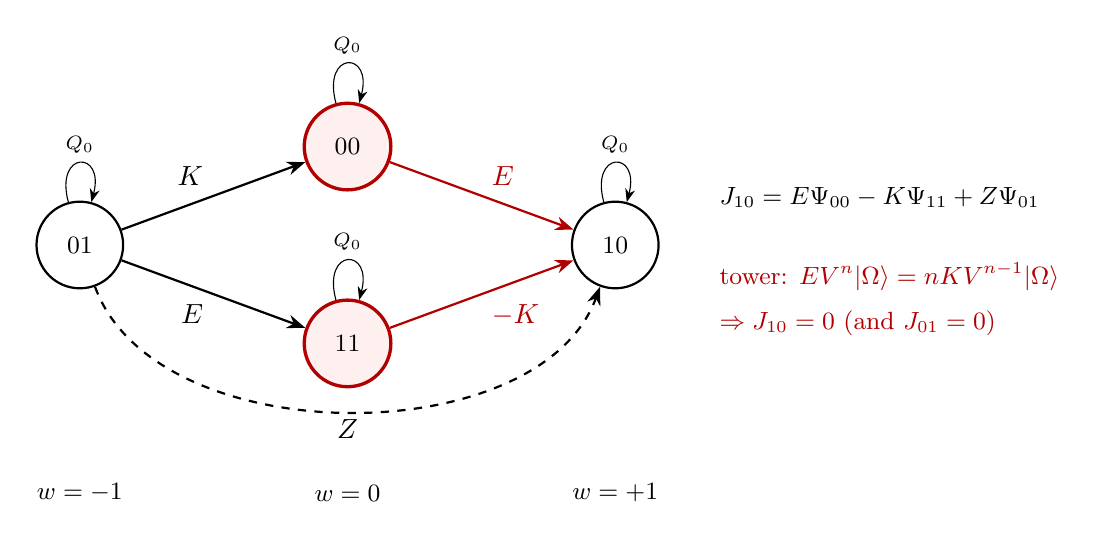
\begin{tikzpicture}[>=Stealth,
  slot/.style={circle,draw,thick,minimum size=11mm,font=\small},
  tow/.style={circle,draw=red!70!black,very thick,fill=red!6,minimum size=11mm,font=\small}]
\node[slot] (s01) at (0,0) {01};
\node[tow]  (s00) at (3.4,1.25) {00};
\node[tow]  (s11) at (3.4,-1.25) {11};
\node[slot] (s10) at (6.8,0) {10};
\draw[->,thick] (s01) -- node[above left]{$K$} (s00);
\draw[->,thick] (s01) -- node[below left]{$E$} (s11);
\draw[->,thick,red!70!black] (s00) -- node[above right]{$E$} (s10);
\draw[->,thick,red!70!black] (s11) -- node[below right]{$-K$} (s10);
\draw[->,thick,dashed] (s01) to[out=-70,in=-110,looseness=0.9] node[pos=0.5,below=-1pt]{$Z$} (s10);
\foreach \s in {s01,s00,s11,s10} \draw[->] (\s) edge[loop above,looseness=6,min distance=6mm] node[above,font=\scriptsize]{$Q_0$} (\s);
\node[font=\small] at (0,-3.15) {$w=-1$};
\node[font=\small] at (3.4,-3.15) {$w=0$};
\node[font=\small] at (6.8,-3.15) {$w=+1$};
\node[font=\small,align=left,anchor=west] at (8.0,0.6) {$J_{10}=E\Psi_{00}-K\Psi_{11}+Z\Psi_{01}$};
\node[font=\small,align=left,anchor=west,red!70!black] at (8.0,-0.4) {tower: $E V^n\Om=nK V^{n-1}\Om$};
\node[font=\small,align=left,anchor=west,red!70!black] at (8.0,-1.0) {$\Rightarrow J_{10}=0$ (and $J_{01}=0$)};
\end{tikzpicture}
\caption{The four slots of the pair uplift, ordered by $w=t_\psi-t_\chi$, and the parts of
$Q_{N+1}=Q_0+\psie^\dagger E+K\chif+\psie^\dagger Z\chif$ connecting them; $Q_0$ acts within each slot. The adjoint
flows into slot 01 form the current $J_{01}$. All dressing is sourced by these arrows. The tower (red) occupies slots 00
and 11 only. Its two arrows into slot 10 cancel by the protection identity $[E,V]=K$, and the adjoint arrows into 01
cancel as well, so the tower needs no dressing at all.}\label{fig:slots}
\end{figure}

\begin{table}[ht]
\centering\small
\caption{Notation.}\label{tab:notation}
\begin{tabular}{@{}>{\raggedright\arraybackslash}p{0.28\textwidth}>{\raggedright\arraybackslash}p{0.66\textwidth}@{}}\toprule
Symbol & Meaning\\\midrule
$(a,b)$, $(A,B)$ & old and new sectors $(N_\psi,N_\chi)$\\
$T=(t_\psi,t_\chi)$; $\Psi_T$ & slot (channel) of the new pair; slot component, a state of the old model\\
$Q_0$, $H_0$, $G=H_0^+$ & old supercharge, Hamiltonian, Green's operator $\int_0^\infty\!d\tau\,e^{-\tau H_0}$ (non-harmonic part)\\
$\B(a,b)$, $b(a,b)$, $\PH$ & old BPS space, its dimension, its projector\\
$E$, $K$, $Z$ & couplings to the new pair, eq.~\eqref{eq:EKZ}\\
$J_{10}$, $J_{01}$ & slot currents, eq.~\eqref{eq:currents}\\
$\dnew$ & dimension of the new BPS space in the target sector\\
$D_T$, $U_T$, $\kappa_T$ & CV's decoder $\Pi_T|_{\B_{N+1}}$, minimum fidelity over the fortuitous subspace, dressing cost\\
$R_T$, $A_T$ & constrained room containing $\mathrm{im}\,D_T$; exact-lift locus $\B\cap\mathrm{im}\,D_T$\\
bare; bare fraction $\mu$ & all slot components old-harmonic; $\sum_T\|\PH\Psi_T\|^2/\|\Psi\|^2$\\\bottomrule
\end{tabular}
\end{table}

%=====================================================================
\section{Adding one mode with an obstruction}\label{sec:onemode}
%=====================================================================

The one-flavor uplift (D6, at half filling) rested on a dimension fact: the image of a harmonic source under the new
couplings lands in a charge sector without cohomology, so it is automatically exact. In the two-flavor model this fails. The targets of
$E$ and $K$ lie inside the window where the old model has BPS states. The following theorem is the replacement.

\begin{theorem}[One added mode with an obstruction]\label{thm:A}\VER\
Let $Q_0$ be nilpotent on a finite-dimensional graded Hilbert space $\Hc_o$. Add one fermionic mode $\mu$, with
$Q=Q_0+\mu^\dagger E$, where $E$ is even and $[Q_0,E]=0$ (``creation type''). Write $\Psi=a+\mu^\dagger b$ with
$a,b\in\Hc_o$, and Hodge-decompose $a=h+x$ and $b=g+z$ ($h,g$ harmonic, $x$ exact, $z$ coexact).
\begin{enumerate}\itemsep2pt
\item[(a)] $\Psi$ is BPS if and only if $Q_0a=0$, $Q_0^\dagger b=0$, $Q_0b=Ea$ and $Q_0^\dagger a=-E^\dagger b$.
\item[(b)] For given harmonic sources $(h,g)$ a BPS state exists if and only if
  \begin{equation}\label{eq:obstruction}
  \PH E\,h=0\qquad\text{and}\qquad \PH E^\dagger g=0 .
  \end{equation}
  It is then unique, with $z=Q_0^+E(h+x)$ and $x=-(Q_0^\dagger)^+E^\dagger(g+z)$.
\item[(c)] Hence $\B\cong\ker(\PH E\PH|_{\B_a})\oplus\ker(\PH E^\dagger\PH|_{\B_b})$. The BPS space splits orthogonally
  as $\B=\B_h\oplus\B_g$ (no harmonic part in the occupied, resp.\ empty, slot), and $\Psi(h,0)$ is the unique
  minimum-norm BPS state whose empty-slot harmonic part is $h$.
\end{enumerate}
For an annihilation-type mode, $Q=Q_0+K\mu$, the roles of the slots are exchanged. Then $a=h+z$ and $b=g+x$, and the
obstructions are $\PH Kg=0$ and $\PH K^\dagger h=0$.
\end{theorem}
\begin{proof}
(a) $Q\Psi=Q_0a+\mu^\dagger(Ea-Q_0b)$ and $Q^\dagger\Psi=Q_0^\dagger a+E^\dagger b-\mu^\dagger Q_0^\dagger b$.

(b) The equation $Q_0b=Ea$ requires $Ea$ to be exact. Now $Ex=EQ_0w=Q_0Ew$ is exact. $Eh$ is closed, because
$Q_0Eh=EQ_0h=0$, and closed forms are harmonic $\oplus$ exact. So $Ea$ is exact if and only if $\PH Eh=0$. Then
$Q_0z=Ea$ has the unique coexact solution $z=Q_0^+Ea$. The coclosed equation is the mirror image. The remaining linear
system for $(x,z)$, given $(h,g)$, is the one of D6~\S5. Its proof uses only $[Q_0,E]=0$ and the exactness of $Ea$, so
it carries over verbatim. The coupling is anti-Hermitian, so $1+\mathbb L$ is invertible and the solution is unique.

(c) The orthogonality of $\Psi(h,0)$ and $\Psi(0,g)$, and the minimum-norm property, follow as in D6 (Theorem~2 and
Corollary~1 of~\cite{prog1013}).
\end{proof}

\begin{remark}[Cohomological reading]
$Q$ is the mapping cone of $E:(\Hc_o,Q_0)\to(\Hc_o,Q_0)$. Its long exact sequence is CV's eq.~(24), with connecting map
$\delta=[E]$, and the dimension count in (c) is CV's eq.~(26). In the half-filling sector of the one-flavor model
used in D6, $\delta=0$ because its target lies outside the fortuity window. (In other one-flavor sectors $\delta$ can be
nonzero; CV \S4.2 show that the incoming and outgoing maps cannot both be.) Theorem~\ref{thm:A} is the harmonic, metric
refinement for $\delta\neq0$.
It gives the explicit uplift map, the obstruction~\eqref{eq:obstruction} on harmonic sources, the orthogonal splitting
and the canonical uplift. CV \S4.3 emphasized that these require ``the Hilbert-space metric and the coupling-dependent
supercharge of the enlarged theory.''
\end{remark}

\VER\ We checked Theorem~\ref{thm:A} at $N=4,5$ in both models by solving the BPS conditions for the non-harmonic parts
with prescribed harmonic sources:
\begin{itemize}\itemsep2pt
\item admissible sources give a BPS state with residual $\le10^{-12}$, with no rank deficit;
\item obstructed sources give residual $\ge1$;
\item the splitting holds to $10^{-13}$.
\end{itemize}

%=====================================================================
\section{The pair uplift}\label{sec:pair}
%=====================================================================

\paragraph{Two obstructed steps.} We add $\psie$ first and $\chif$ second.
\begin{itemize}\itemsep2pt
\item Step 1 is of creation type with the operator $E$. It produces an intermediate model $M$, in which $\chif$ is
  frozen empty and $Q_M=Q_0+\psie^\dagger E$.
\item Step 2 is of annihilation type over $M$, with $K'=K+\psie^\dagger Z$. The required $[Q_M,K']=0$ is
  equation~\eqref{eq:nil}.
\end{itemize}
Theorem~\ref{thm:A} applied twice gives the BPS space of the enlarged model explicitly, and in particular
\begin{align}
\dim\B_M(A,B)&=\dim\ker\big(\PH E\PH\big|_{\B(A,B)}\big)+\dim\ker\big(\PH E^\dagger\PH\big|_{\B(A-1,B)}\big),\label{eq:dimM}\\
\dim\B_{N+1}(A,B)&=\dim\ker\big(\PH K'^\dagger\PH\big|_{\B_M(A,B)}\big)+\dim\ker\big(\PH K'\PH\big|_{\B_M(A,B-1)}\big).\label{eq:dimN}
\end{align}
\VER\ There are no mismatches in any sector for $N=2$--$7$: $950$ symmetrized and $570$ generic sector records for
$N\le6$, plus 81 sector records (seed 1) at $N=7$.

\paragraph{The four-slot harmonic map.} \NUM\ A BPS state whose four slot components all have vanishing old-harmonic part
is zero. Equivalently, $\B_{N+1}(A,B)$ embeds in $\bigoplus_T\B(\text{slot }T)$. We find no rank deficit for any sector
at $N=2$--$7$ in either model, and every BPS state is reconstructed from its four harmonic slot parts to $10^{-14}$. We
have no proof. The obstacle is that the old-harmonic part of $\Psi_{00}$ is $h_{00}+\PH E^\dagger d$, where $d$ comes
from the $M$-coexact dressing of step~2, rather than the step-1 source $h_{00}$ itself. Injectivity is not
robust, though. The smallest eigenvalue of the operator~\eqref{eq:G} below falls to $1.8\times10^{-6}$ (seed 1) and
$5\times10^{-5}$ (generic) in sectors $(3,3)$ and $(5,5)$ at $N=7\to8$. \emph{Update (\S\ref{sec:unique}):} this happens
where the old model has a near-zero mode. Injectivity is generic, but it fails exactly on a codimension-two set of
couplings, where pure-dressing BPS states exist. Where it holds, injectivity makes the following operator positive
definite on $\B_{N+1}$:
\begin{equation}\label{eq:G}
\mathcal G=\sum_T S_T^\dagger\,\PH\,S_T\qquad(S_T:\ \text{slot-}T\text{ component}).
\end{equation}
Its eigenvalue on a state is the \emph{bare fraction} $\mu\in(0,1]$: the share of the norm carried by old BPS states
in the four slots. A state is \emph{bare} if $\mu=1$, i.e.\ if its Hodge dressing vanishes. In the one-flavor model, at
first order, $\mu=1/(1+\sigma^2)$ coincides with the decoder eigenvalue $\lambda$ on the $h$ family and with $1-\lambda$
on the $g$ family. $\mathcal G$ is the slot-symmetric version of that quantity, and it is the natural object when there
are four slots.

\paragraph{Old cohomology plus $[E],[K]$ is not enough.} Because the pair has three filtration levels, one may try to
compute $\B_{N+1}$ from the \emph{slot complex} of old BPS data,
\begin{equation}\label{eq:slotcomplex}
\B(01)\ \xrightarrow{\ ([K],[E])\ }\ \B(00)\oplus\B(11)\ \xrightarrow{\ [E]\,h_{00}-[K]\,h_{11}\ }\ \B(10).
\end{equation}
This is the $E_1$ page of the spectral sequence of the $w$ filtration, and $d_1^2=[\{Q_0,Z\}]=0$. Its cohomology $E_2$
bounds $\dim\B_{N+1}$ from above. \NUM\ The bound is saturated in all sectors but four per $N$, identically in both
models (Table~\ref{tab:d2}). There a differential $d_2\sim[Z-EQ_0^+K+KQ_0^+E]$ pairs the $w=-1$ classes of sector
$(A,B)$ with the $w=+1$ classes of $(A+2,B-1)$. So the pair uplift is \emph{not} determined by the old BPS data and the
first-order maps alone. The two-step formula~\eqref{eq:dimN} is exact and accounts for $d_2$.

\begin{table}[ht]
\centering\small
\caption{The four sectors per $N$ where the slot complex~\eqref{eq:slotcomplex} overcounts: $\dim E_2\to\dim\B_{N+1}$.
In every case $E_2$ sits entirely at $w=-1$ (sectors with $A<B$) or at $w=+1$ (sectors with $A>B$). $d_2$ maps
sector $(A,B)$ to $(A+2,B-1)$ with the maximal rank: 9, 78, 91 at $N=5,6,7$, for example. Identical in all
realizations of both models.}\label{tab:d2}
\begin{tabular}{@{}cllll@{}}\toprule
$N\to N+1$ & \multicolumn{4}{c}{sector: $\dim E_2\to\dim\B_{N+1}$}\\\midrule
$4\to5$ & $(1,2)$: $10\to2$ & $(2,4)$: $9\to1$ & $(3,1)$: $9\to1$ & $(4,3)$: $10\to2$\\
$5\to6$ & $(1,2)$: $9\to0$ & $(3,1)$: $33\to24$ & $(3,5)$: $33\to24$ & $(5,4)$: $9\to0$\\
$6\to7$ & $(2,3)$: $92\to14$ & $(3,5)$: $78\to0$ & $(4,2)$: $78\to0$ & $(5,4)$: $92\to14$\\
$7\to8$ & $(2,3)$: $91\to0$ & $(4,2)$: $330\to239$ & $(4,6)$: $330\to239$ & $(6,5)$: $91\to0$\\\bottomrule
\end{tabular}
\end{table}

%=====================================================================
\section{The tower: protection by current cancellation}\label{sec:tower}
%=====================================================================

\begin{proposition}[The tower is bare]\label{prop:tower}\VER\
In the symmetrized model, the enlarged tower state $V_{N+1}^n\Om$ has slot components
\begin{equation}\label{eq:towerslots}
\Psi_{00}=V^n\Om,\qquad \Psi_{11}=n\,V^{n-1}\Om,\qquad \Psi_{10}=\Psi_{01}=0,
\end{equation}
all of them old BPS states. Both slot currents vanish, and the tower has bare fraction $\mu=1$ at every $N$. Its slot
weights are $(N+1-n)/(N+1)$ in 00 and $n/(N+1)$ in 11.
\end{proposition}
\begin{proof}
Equation~\eqref{eq:towerslots} is CV's eq.~(85). The operator $\psie^\dagger\chif^\dagger$ squares to zero and
commutes with $V_N$, so the binomial expansion of $(V_N+\psie^\dagger\chif^\dagger)^n$ stops after one term. Both
components are old BPS states. From~\eqref{eq:ward} and $E\Om=0$,
\begin{equation}\label{eq:EVn}
E\,V^n\Om=\sum_{m}V^m[E,V]V^{n-1-m}\Om=n\,K\,V^{n-1}\Om ,
\end{equation}
so $J_{10}=EV^n\Om-nKV^{n-1}\Om=0$. For $J_{01}$, compute $Q_{N+1}^\dagger V_{N+1}^n\Om=\chif^\dagger J_{01}$, using
$Q_0^\dagger V^m\Om=0$. The left side vanishes by CCSY (3.23) at size $N+1$. The remaining six equations of
Table~\ref{tab:slots} hold trivially for harmonic $\Psi_{00}$, $\Psi_{11}$. The weights follow from CV (86):
$n^2\|V^{n-1}\Om\|^2/\|V^n_{N+1}\Om\|^2=n/(N+1)$.
\end{proof}

\VER\ The bare fraction equals 1, and the slot weights agree to $4\times10^{-16}$, for all $n$ at $N=2$--$7$.

\paragraph{Reading.} \INTERP\ The current $J_{10}$ is what the old model must absorb when a state in slot 00 is
promoted, $Q_0\Psi_{10}=J_{10}$. A fortuitous state must absorb it with a Hodge dressing cloud. The tower instead pays
with a second old BPS state: the 11 component $nV^{n-1}\Om$, whose $K$-image cancels the $E$-image of the 00 component.
The cancellation is the Ward identity of $V$. The tower's uplift is fixed by symmetry and involves no dynamics of the old
model.

\paragraph{Two notions of dressing.} CV call~\eqref{eq:towerslots} ``genuinely dressed'' ($\kappa_{00}>0$), because
relative to the 00 channel the state needs its 11 component. In Hodge terms it has no dressing at all. Both statements are
correct. CV's dressing measures support outside one channel; the Hodge dressing measures non-BPS content in any slot.
This report says \emph{bare} for the latter. The tower is not an eigenvector of CV's slot decoders $P\Pi_TP$: the
residuals $\|P\Pi_TP\,t-\lambda t\|$ (with $\lambda=\ip{t}{P\Pi_TPt}$ the slot weight) are $0.12$--$0.43$ for
$N=5\to6$ through $7\to8$, and equal for $T=00$ and $11$ because $P\Pi_{10}Pt=P\Pi_{01}Pt=0$.

%=====================================================================
\section{Bare states: arithmetic walls and the tower excess}\label{sec:bare}
%=====================================================================

\paragraph{The bare map.} With all four $\Psi_T=h_T$ harmonic, Table~\ref{tab:slots} reduces to:
\begin{itemize}\itemsep2pt
\item $Kh_{01}=0$ and $Eh_{01}=0$;
\item $E^\dagger h_{10}=0$ and $K^\dagger h_{10}=0$;
\item $J_{10}=Eh_{00}-Kh_{11}+Zh_{01}=0$ and $J_{01}=K^\dagger h_{00}+E^\dagger h_{11}+Z^\dagger h_{10}=0$.
\end{itemize}
The bare BPS states are the kernel of this linear map on $\bigoplus_T\B(\text{slot }T)$. Each equation lives in a known
constrained space. $Kh_{01}$ is closed in $(A+2,B-1)$, $Eh_{01}$ closed in $(A+1,B-2)$, $E^\dagger h_{10}$ and
$K^\dagger h_{10}$ coclosed in $(A-2,B+1)$ and $(A-3,B)$. $J_{10}$ is closed in $(A+1,B-1)$ once $Kh_{01}=Eh_{01}=0$,
because $Q_0J_{10}=[E,K]h_{01}$; $J_{01}$ is coclosed in $(A-2,B)$ by the mirror argument.

\paragraph{Generic count.} Placing each equation in generic position inside its constrained space gives
$n_{01}=\max(0,b_{01}-c_1-c_2)$ and $n_{10}=\max(0,b_{10}-c_3-c_4)$ for the slot-01 and slot-10 kernels, where the
$c$'s are the dimensions of the constrained spaces. The count is then
\begin{equation}\label{eq:baregen}
\text{bare}_{\rm gen}=\max\big(0,\ b_{00}+b_{11}+n_{01}+n_{10}-c(J_{10})-c(J_{01})\big).
\end{equation}

\paragraph{Result.} \NUM\ The law
\begin{equation}\label{eq:barelaw}
\#\text{bare}=\text{bare}_{\rm gen}+\big[\,1\ \text{in diagonal sectors }(n,n),\,1\le n\le N,\ \text{where}\ \text{bare}_{\rm gen}=0\,\big]
\end{equation}
holds with no exception in all $400$ symmetrized and $240$ generic sector records at $N=2$--$6$, and at $N=7$
(Table~\ref{tab:bare}). This uses the exact dimensions of the two sub-kernels $n_{01}$, $n_{10}$. Their generic values fail
by one at $N=5$ only (see below). The bracket is the tower. The excess first appears at $N=6\to7$ in the central sectors
$(3,3)$ and $(4,4)$, and at $N=7\to8$ in \emph{every} diagonal sector. The generic model never has an excess. Its bare
states, the \emph{arithmetic walls}, coincide in number with those of the symmetrized model in every sector
(Fig.~\ref{fig:bare}).

\begin{table}[ht]
\centering\small
\caption{Bare BPS states vs.\ the generic count~\eqref{eq:baregen}, seed 1 (other seeds identical). Sectors not listed
have neither. ``tower'': the excess state is the tower; the generic model has $0$ there.}\label{tab:bare}
\begin{tabular}{@{}ll@{}}\toprule
$N\to N+1$ & sector: bare (generic count)\\\midrule
$6\to7$ & $(1,0)$: 7 (7);\ $(1,1)$: 2 (2);\ $(2,0)$: 8 (8);\ $(2,1)$: 41 (41);\ $(2,2)$: 3 (3);\ $(3,2)$: 25 (25);\\
 & $(3,3)$: \textbf{1 (0) tower};\ $(4,4)$: \textbf{1 (0) tower};\ and mirrors $(A,B)\to(N{+}1{-}A,N{+}1{-}B)$\\
$7\to8$ & $(1,0)$: 8 (8);\ $(1,1)$: \textbf{1 (0) tower};\ $(2,0)$: 13 (13);\ $(2,1)$: 56 (56);\ $(2,2)$: \textbf{1 (0) tower};\\
 & $(3,1)$: 7 (7);\ $(3,2)$: 50 (50);\ $(3,3)$, $(4,4)$: \textbf{1 (0) tower} each;\ and mirrors\\\bottomrule
\end{tabular}
\end{table}

\begin{figure}[ht]
\centering
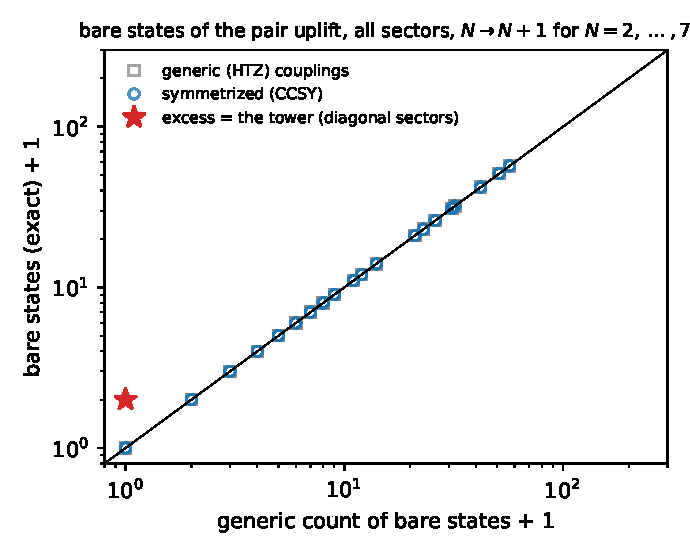
\includegraphics[width=0.62\textwidth]{progress_2026-10-23_figs/fig_bare_counts.pdf}
\caption{Bare BPS states of the pair uplift against the generic count~\eqref{eq:baregen}, for all sectors and
realizations at $N=2\to3,\dots,7\to8$. Symmetrized (circles) and generic (squares) couplings coincide everywhere. The only
points off the diagonal are the tower (stars): a bare state in a diagonal sector where the count predicts none.
\NUM}\label{fig:bare}
\end{figure}

\paragraph{The $N=5$ coincidences.} \NUM\ At $N=5$, and only there among $N=2$--$7$, three generic-position counts fail
by one dimension. All three failures occur in both models and in all seeds. The old-model gaps are clean (zero modes
$\le10^{-13}$, gaps $\ge0.03$), so these are not tolerance artifacts.
\begin{enumerate}\itemsep2pt
\item $\dim\ker[E^\dagger;K^\dagger]$ on $\B(2,2)$, and its mirror $\ker[K;E]$ on $\B(3,3)$.
\item $\ker[K;E]$ on $\B(2,1)$, and its mirror $\ker[E^\dagger;K^\dagger]$ on $\B(3,4)$.
\item $\B(2,2)\cap(\mathrm{im}\,D_{01})^\perp$, and its mirror (\S\ref{sec:cv}).
\end{enumerate}
The extra vector in item~3 is not the one in item~1 (overlap $4$--$6\,\%$). We have no explanation. They recall the
unexplained ``atom excess'' of the one-flavor model (D6~\S4).

\paragraph{Monotone vs.\ fortuitous at the level of bare states.} Every bare fortuitous state is an arithmetic wall. Walls
are determined by counting, identical for generic couplings, and confined at $N=7\to8$ to the peripheral sectors
$(1,0)$, $(2,0)$, $(2,1)$, $(3,1)$, $(3,2)$ and their mirrors. The tower is the only bare state the counting does not
produce.

%=====================================================================
\section{CV's channel decoders: rooms and generic position}\label{sec:cv}
%=====================================================================

CV's decoder for channel $T$ maps an enlarged BPS state to its slot-$T$ component, $D_T=\Pi_T|_{\B_{N+1}}$. An old BPS
state $\alpha$ lifts exactly through $T$ if $\alpha\in\mathrm{im}\,D_T$. The \emph{exact-lift locus} is
$A_T=\B\cap\mathrm{im}\,D_T$, and $U_T$ is the minimum fidelity $\|P_{\mathrm{im}\,D_T}\alpha\|^2$ over the unit
fortuitous states (CV eqs.~44, 50, 89).

\subsection{Constrained rooms}\label{sec:rooms}

CV \S7.1 explained the one-flavor exact-lift loci by placing $\B$ and $\mathrm{im}\,D_T$ in generic position inside a
constrained ``room'', the kernel of $Q_N$ or $Q_N^\dagger$. Table~\ref{tab:slots} gives the analogous rooms for the four
channels. \DER\ For the old sector $(a,b)$:
\begin{align}
R_{01}&=\ker Q_0,\qquad R_{10}=\ker Q_0^\dagger,\nonumber\\
R_{00}&=\B(a,b)\oplus Q_0^+K\big(\ker Q_0|_{(a,b-1)}\big)\oplus(Q_0^\dagger)^+E^\dagger\big(\ker Q_0^\dagger|_{(a-1,b)}\big),\label{eq:rooms}\\
R_{11}&=\B(a,b)\oplus Q_0^+E\big(\ker Q_0|_{(a+1,b)}\big)\oplus(Q_0^\dagger)^+K^\dagger\big(\ker Q_0^\dagger|_{(a,b+1)}\big).\nonumber
\end{align}
For 01 and 10 this is the closedness of $\Psi_{01}$ and the coclosedness of $\Psi_{10}$. For 00 it follows from the first
row of Table~\ref{tab:slots}. The coexact part of $\Psi_{00}$ is $-Q_0^+K\Psi_{01}$ with $\Psi_{01}$ closed, and its
exact part is $-(Q_0^\dagger)^+E^\dagger\Psi_{10}$ with $\Psi_{10}$ coclosed. Channel 11 follows likewise.

\subsection{Two counting laws}

\begin{law}[rank]\label{law:L1}\NUM\ $\rk D_T=\min(\dnew,R_T)$, with $\dnew=\dim\B_{N+1}$ of the target sector.\end{law}
\begin{law}[exact-lift locus]\label{law:L2}\NUM\ $\dim A_T=\max(0,\ b+\rk D_T-R_T)$.\end{law}
Both laws hold with no exception in $1300$ (sector, channel, seed) records of the symmetrized model and $780$ of the
generic model at $N=2$--$6$, and in the further $176$ and $88$ records at $N=7$. They imply three corollaries for the fortuitous subspace
$F$, of dimension $f$:
\begin{itemize}\itemsep2pt
\item[(C1)] $U_T=1$ if and only if $\dnew\ge R_T$. On the diagonal this uses the fact that the tower lies in $A_{00}$ and
  $A_{11}$.
\item[(C2)] $U_T=0$ if and only if $F\cap(\mathrm{im}\,D_T)^\perp\ne0$. The generic count is
  $b-\rk D_T>0$ for the channels 00 and 11 on the diagonal, where the tower is protected, and $f-\rk D_T>0$ otherwise.
\item[(C3)] $0<U_T<1$ in all remaining cases.
\end{itemize}

\subsection{CV's Fig.~6, reproduced and explained}

Figure~\ref{fig:cv} shows $U_T$ for the fortuitous subspaces in CV's eleven sectors at $N=2\to3,\dots,7\to8$, computed with
our code, together with the category predicted by (C1)--(C3). \NUM\ The observations are:
\begin{itemize}\itemsep2pt
\item The 0/1 pattern is CV's. The intermediate values agree within realization scatter, e.g.\ $(1,2)$/00 at
  $3\to4$: $0.30$ here, $0.45$ in CV.
\item The predicted category agrees with the observation in every cell and every seed of the symmetrized model.
\item In the generic control, the categories fail only at $N=5$ in $(2,2)$/01 and its mirror (coincidence~3 above).
\end{itemize}
Some intermediate values coincide, e.g.\ $(1,2)$/00 and $(2,1)$/11 at $3\to4$, in CV's table as well. These are
particle--hole symmetry, $(a,b;T)\leftrightarrow(N-a,N-b;\bar T)$, acting realization by realization.

CV's qualitative summary reads ``the charge-preserving channel 00 fails for the $\chi$-heavy sectors, whereas those sectors
lift perfectly through the $+\psi$ channel''. In our terms it is the inequality $\dnew\ge R_T$, sector by sector.
Table~\ref{tab:chiheavy} shows the numbers for the $\chi$-heavy rows. For $\chi$-heavy sectors, $+\psi$ moves the
target toward the diagonal, where BPS states are plentiful, so $\dnew$ exceeds the room. The 00 channel keeps the
charge, and its target BPS space falls below the room as $N$ grows.

\begin{figure}[p]
\centering
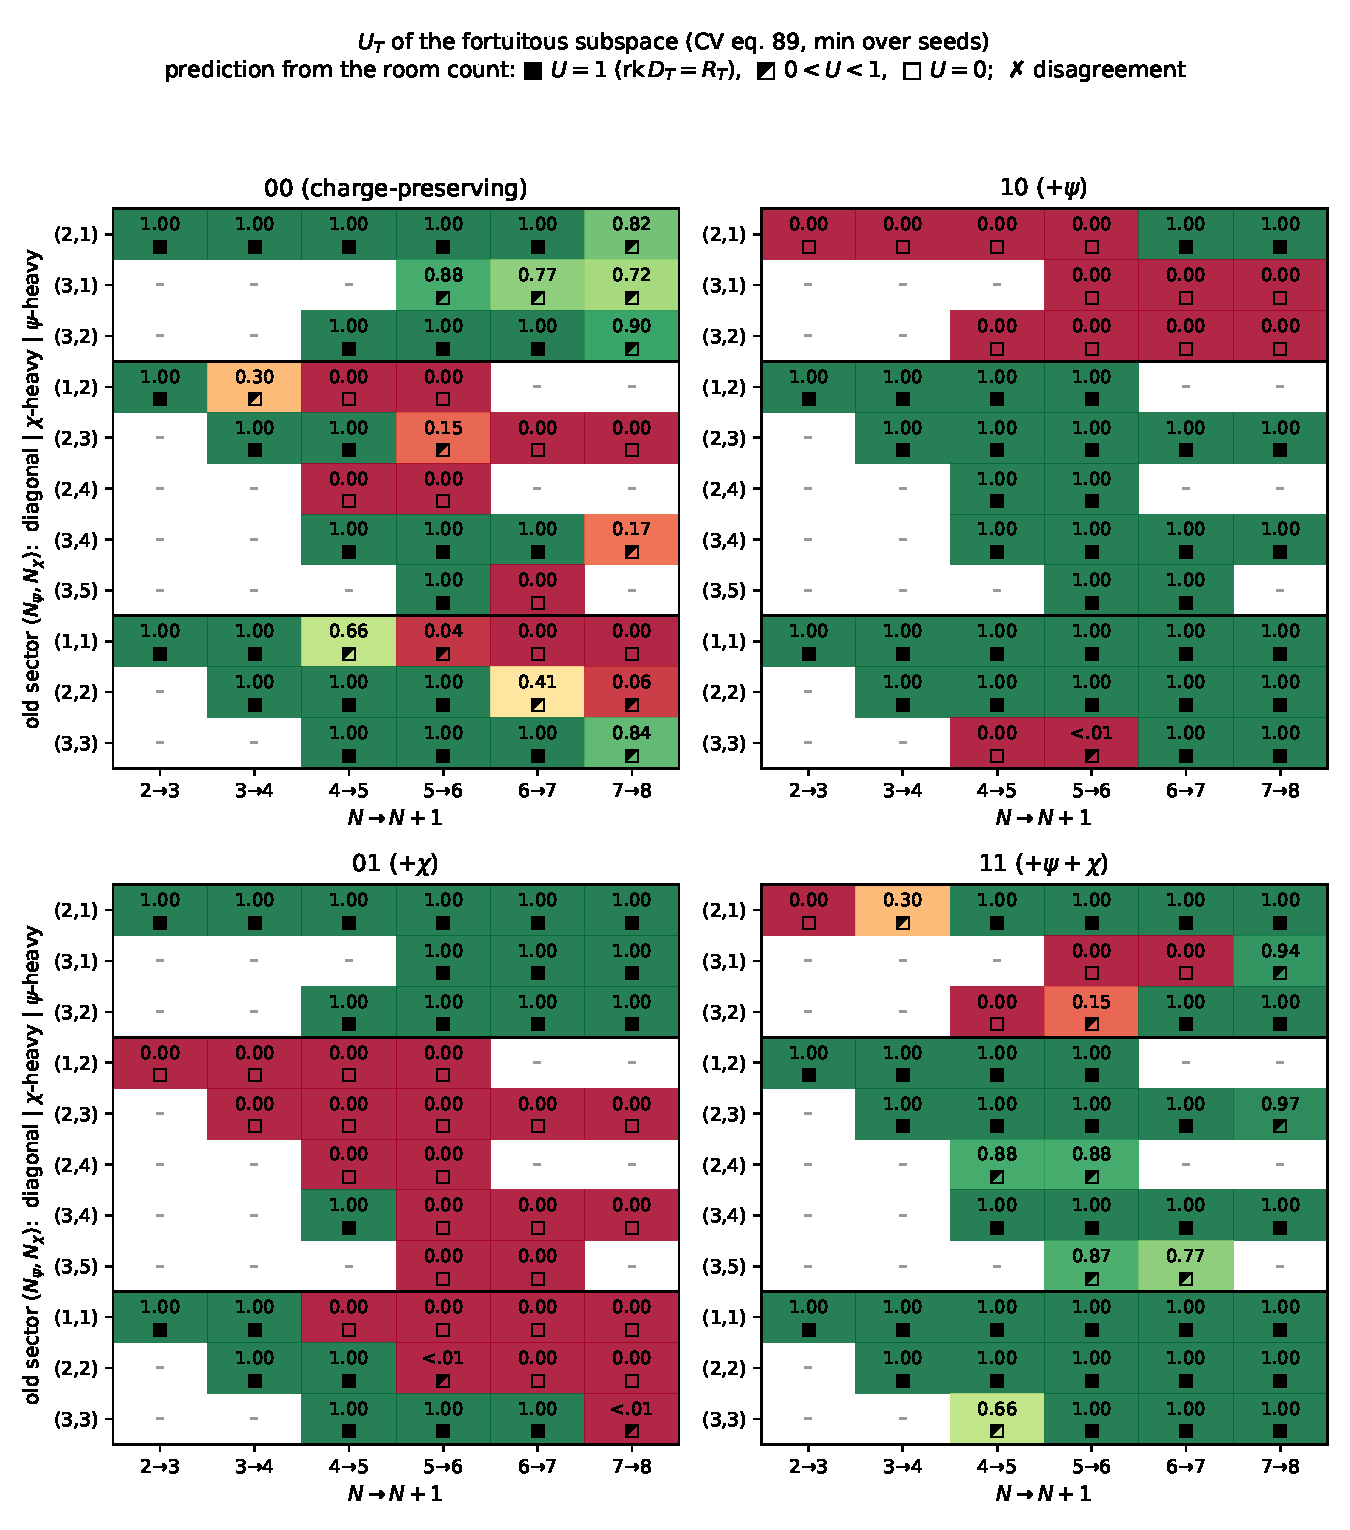
\includegraphics[width=\textwidth]{progress_2026-10-23_figs/fig_cv_fidelity.pdf}
\caption{CV's Fig.~6 recomputed: $U_T$ of the fortuitous subspace by sector (rows) and channel (panels), minimum over
seeds (five for $N\le6$, two for $N=7$). Symbols give the category predicted by Laws~\ref{law:L1}--\ref{law:L2}:
$\blacksquare$ $U=1$ ($\rk D_T=R_T$), half-filled $0<U<1$, $\square$ $U=0$. No cell disagrees. ``$<.01$'' marks small
positive values.}\label{fig:cv}
\end{figure}

\begin{table}[ht]
\centering\small
\caption{The mechanism behind CV's $\chi$-heavy rows (seed 1, $N=3$--$7$): target BPS dimension $\dnew$ vs.\ room
$R_T$, the exact-lift codimension $b-\dim A_T$, and $U_T$. $U_T=1$ exactly when $\dnew\ge R_T$.}\label{tab:chiheavy}
\begin{tabular}{@{}cc|cccc|cccc@{}}\toprule
& & \multicolumn{4}{c|}{channel 00} & \multicolumn{4}{c}{channel 10 ($+\psi$)}\\
$N$ & sector & $\dnew$ & $R_{00}$ & codim & $U$ & $\dnew$ & $R_{10}$ & codim & $U$\\\midrule
3 & $(1,2)$ & 8 & 9 & 1 & 0.39 & 28 & 9 & 0 & 1\\
3 & $(2,3)$ & 17 & 3 & 0 & 1 & 12 & 3 & 0 & 1\\
4 & $(1,2)$ & 2 & 20 & 8 & 0 & 65 & 24 & 0 & 1\\
4 & $(2,3)$ & 45 & 24 & 0 & 1 & 65 & 23 & 0 & 1\\
4 & $(2,4)$ & 1 & 6 & 2 & 0 & 35 & 6 & 0 & 1\\
4 & $(3,4)$ & 35 & 4 & 0 & 1 & 15 & 4 & 0 & 1\\
5 & $(1,2)$ & 0 & 17 & 2 & 0 & 116 & 50 & 0 & 1\\
5 & $(2,3)$ & 66 & 100 & 34 & 0.30 & 220 & 95 & 0 & 1\\
5 & $(2,4)$ & 0 & 47 & 1 & 0 & 144 & 49 & 0 & 1\\
5 & $(3,4)$ & 144 & 50 & 0 & 1 & 116 & 45 & 0 & 1\\
5 & $(3,5)$ & 24 & 10 & 0 & 1 & 60 & 10 & 0 & 1\\
6 & $(2,3)$ & 14 & 217 & 66 & 0 & 546 & 285 & 0 & 1\\
6 & $(3,4)$ & 364 & 300 & 0 & 1 & 546 & 264 & 0 & 1\\
6 & $(3,5)$ & 0 & 120 & 24 & 0 & 344 & 114 & 0 & 1\\
7 & $(2,3)$ & 0 & 252 & 14 & 0 & 1072 & 700 & 0 & 1\\
7 & $(3,4)$ & 560 & 1205 & 364 & 0.21 & 1820 & 1078 & 0 & 1\\
\bottomrule
\end{tabular}
\end{table}

\subsection{The tower in CV's channels, and its dressing cost}\label{sec:towercost}

The tower lies in $A_{00}$ and $A_{11}$ for every $N$: a specific vector of $\B$ lies in a subspace of positive
codimension, so it is not in generic position. Yet $\dim A_T$ still equals the generic count; the tower is one of its
directions. In the single-mode channels the tower behaves like any vector of $\B$. Its fidelities there are reproduced
together with CV's Fig.~7 (their eq.~90 is again particle--hole symmetry).

CV's dressing cost is $\kappa_T(\alpha)=\|D_T^+\alpha\|^2/\|\alpha\|^2-1$, with $D_T^+\alpha$ the minimum-norm exact
uplift. For the tower, (85) supplies one uplift with cost $n/(N+1-n)$ in channel 00 (CV 87) and $(N-n)/(n+1)$ in channel
11 (CV 88). The minimum-norm uplift is the tower minus its projection onto $\ker D_T$, so the cost reaches the bound if
and only if the tower is orthogonal to $\ker D_T$. \NUM\ In all $255$ (rung, channel, seed) records at $N=2$--$7$, the bound is attained \emph{exactly when} $\ker D_T=0$, and the cost lies strictly below it otherwise
(Fig.~\ref{fig:towercost}). Combined with Law~\ref{law:L1}, $\ker D_T=0\iff\dnew\le R_T$, so
\begin{equation}\label{eq:towercost}
\begin{aligned}
\kappa_{00}(V^n\Om)=\frac{n}{N+1-n}\quad&\iff\quad \dnew(n,n)\le R_{00}(n,n),\\
U_{00}(n,n)=1\quad&\iff\quad \dnew(n,n)\ge R_{00}(n,n).
\end{aligned}
\end{equation}
\textbf{The tower's cost locks onto CV's bound exactly when the charge-preserving channel stops lifting every fortuitous
state of the sector}; both happen at $\dnew=R_{00}$ when equality holds. This explains CV's observation that the cost
``rises onto [the bound] only once $N\gtrsim n+3$''. Here $n=1$ is at the bound from $N=4$, $n=2$ from $N=6$, and
$n=3$ from $N=7$, while $n=4$ is still below it at $N=7$. Sector $(3,3)$ shows both halves of~\eqref{eq:towercost}
across two sizes. At $N=6\to7$ the tower's cost is below the bound and $U_{00}=1$. At $N=7\to8$ the cost sits on the
bound and $U_{00}=0.84$ (Fig.~\ref{fig:cv}).

\begin{figure}[ht]
\centering
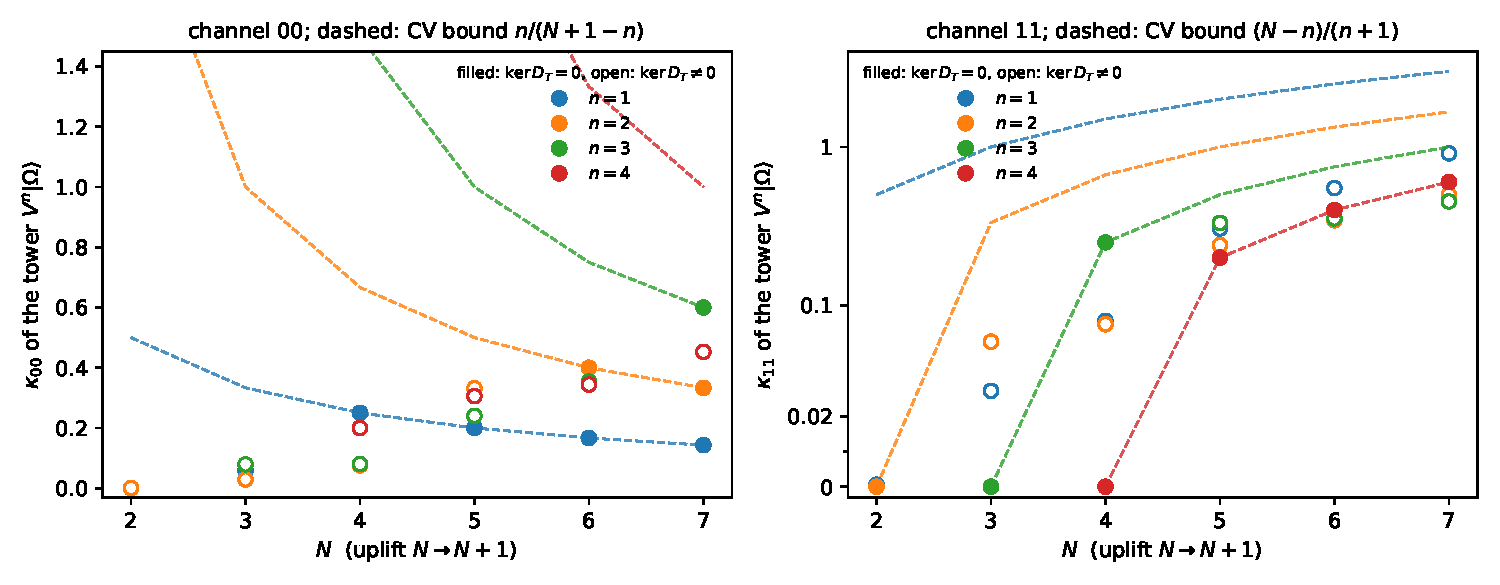
\includegraphics[width=0.95\textwidth]{progress_2026-10-23_figs/fig_tower_costs.pdf}
\caption{CV dressing costs of the tower, computed as exact minimum-norm uplifts (seed 1), against CV's bounds (dashed).
Filled markers: $\ker D_T=0$, where the cost equals the bound. Open: $\ker D_T\ne0$, where it lies below. \NUM}\label{fig:towercost}
\end{figure}

%=====================================================================
\section{First order: dressing as interfering two-point functions}\label{sec:first}
%=====================================================================

\paragraph{First-order dressing.} Replace each $\Psi_T$ by its harmonic source $h_T$ on the right of
Table~\ref{tab:slots}. The six non-harmonic pieces of a BPS state are then
\begin{equation}\label{eq:first}
\begin{aligned}
z_{10}&=Q_0^+J_{10}(h), & x_{01}&=(Q_0^\dagger)^+J_{01}(h),& z_{00}&=-Q_0^+Kh_{01},\\
x_{00}&=-(Q_0^\dagger)^+E^\dagger h_{10},& z_{11}&=-Q_0^+Eh_{01},& x_{11}&=(Q_0^\dagger)^+K^\dagger h_{10}.
\end{aligned}
\end{equation}
The first-order dressing cost $\kappa^{(1)}$ is the sum of their squared norms divided by $\|h\|^2$. The first-order bare
fraction is $1/(1+\kappa^{(1)})$, obtained as a generalized eigenproblem on the admissible sources. As in one flavor,
an exactly bare state has $\kappa^{(1)}=0$, and numerically the converse holds as well.

\paragraph{Single-slot sources: two-point functions.} \VER\ On exact forms $Q_0^+$ has norm-square $\ip{j}{Gj}$, and
likewise $(Q_0^\dagger)^+$ on coexact forms, with $G=H_0^+=\int_0^\infty d\tau\,e^{-\tau H_0}$. Hence a source in one slot
has
\begin{equation}\label{eq:sigmas}
\begin{aligned}
\sigma^2_{00}&=\ip{E h}{GEh}+\ip{K^\dagger h}{GK^\dagger h}, &
\sigma^2_{01}&=\ip{Kh}{GKh}+\ip{Eh}{GEh}+\ip{Zh}{GZh},\\
\sigma^2_{11}&=\ip{Kh}{GKh}+\ip{E^\dagger h}{GE^\dagger h}, &
\sigma^2_{10}&=\ip{E^\dagger h}{GE^\dagger h}+\ip{K^\dagger h}{GK^\dagger h}\\
&&&\quad+\ip{Z^\dagger h}{GZ^\dagger h}.
\end{aligned}
\end{equation}
These hold to $10^{-8}$ (test). Each term is a zero-temperature, Euclidean-time-integrated two-point function in the old
model, between a BPS state and the continuum, of one of three matter operators: flavor conversion $\psi^\dagger\chi$
($E$), $\psi$-pair creation ($K$), or single-$\psi$ creation ($Z$). This generalizes D6's
$\sigma^2\in\mathrm{spec}\,PE^\dagger H_0^{-1}EP$. For terms involving $Z$, $J_{10}$ need not be closed, and the
pseudo-inverse projects first.

\paragraph{Interference.} Sources in several slots share the currents~\eqref{eq:currents}. The dressing therefore
contains cross terms between different matter operators, e.g.\ $-2\,\mathrm{Re}\ip{Eh_{00}}{G\,Kh_{11}}$ from
$\|Q_0^+J_{10}\|^2$. \VER\ The tower is the exactly dark state of this quadratic form: $J_{10}=J_{01}=0$, although its
incoherent single-slot sum is not small. That sum is $0.07$--$6.9$ at $N=5$ and $0.07$--$1.8$ at $N=6$. It varies
between realizations with the old model's gap, which is as small as $0.03$ at $N=5$.

\NUM\ Fortuitous states interfere too (Fig.~\ref{fig:first}b). In the eigenbasis of the exact bare fraction, the ratio
$(\kappa^{(1)}-\kappa_{\rm inc})/\kappa_{\rm inc}$ decreases with $\mu$. It is near $+1$ (constructive) for the most
dressed states and approaches $-1$ (complete cancellation) as $\mu\to1$. At $N=6\to7$ it is close to a single function
of $\mu$. At $N=7\to8$ a second, more destructive branch appears at small $\mu$. Part of this
correlation is variational: the decoder's eigenvectors extremize the dressing form, so extreme $\mu$ goes with extreme
interference. It nevertheless shows that the spread of the bare-fraction spectrum comes largely from interference between
slots, not from the spread of single-slot costs. \textbf{We therefore retract the working hypothesis ``monotone $=$
coherent, fortuitous $=$ incoherent''.} What distinguishes the tower is \emph{exact} cancellation at every $N$, enforced
by an identity, not the presence of interference.

\paragraph{Accuracy.} \NUM\ First order reproduces the exact bare-fraction distribution (Fig.~\ref{fig:first}a). Sector
means agree to within $4.2\,\%$ in all sectors with at least 50 states at $N=5,6$. First order is usually lower,
e.g.\ $0.7014$ vs.\ $0.7322$ in $(3,3)$ at $N=6\to7$, five seeds. The agreement degrades slowly with $N$: at $N=7\to8$
(seed 1) it is $0.6713$ vs.\ $0.7150$ in the central sector $(4,4)$, and all sectors lie within $6.2\,\%$. Walls coincide
in every sector. Exact walls are necessarily first-order walls; the converse is observed, not proved.

\paragraph{Near-bare fortuitous states and the hard edge.} \NUM\ States with $\mu$ close to 1 are numerous at
$N=6\to7$. The fraction with $0.99<\mu<1$ is $0.16$ in the central sectors. There the bare map is nearly square:
$336$ unknowns against $339$ constraints in $(3,3)$, so $\text{bare}_{\rm gen}$ sits three short of threshold. This is
the analogue of D6's hard edge. At $N=7\to8$ the bare map is far from square ($1092$ unknowns against $1428$ constraints
in $(4,4)$), and the near-bare fraction falls to $0.065$ (seed 1). Going down in $N$ it is $0.07$--$0.08$ at $N=5$ and
$0.003$ at $N=4$, where unknowns exceed constraints and exact walls take over. We had seen partial $N=7$ quantiles
before writing this, so it is a consistency check, not a blind test.

\begin{figure}[ht]
\centering
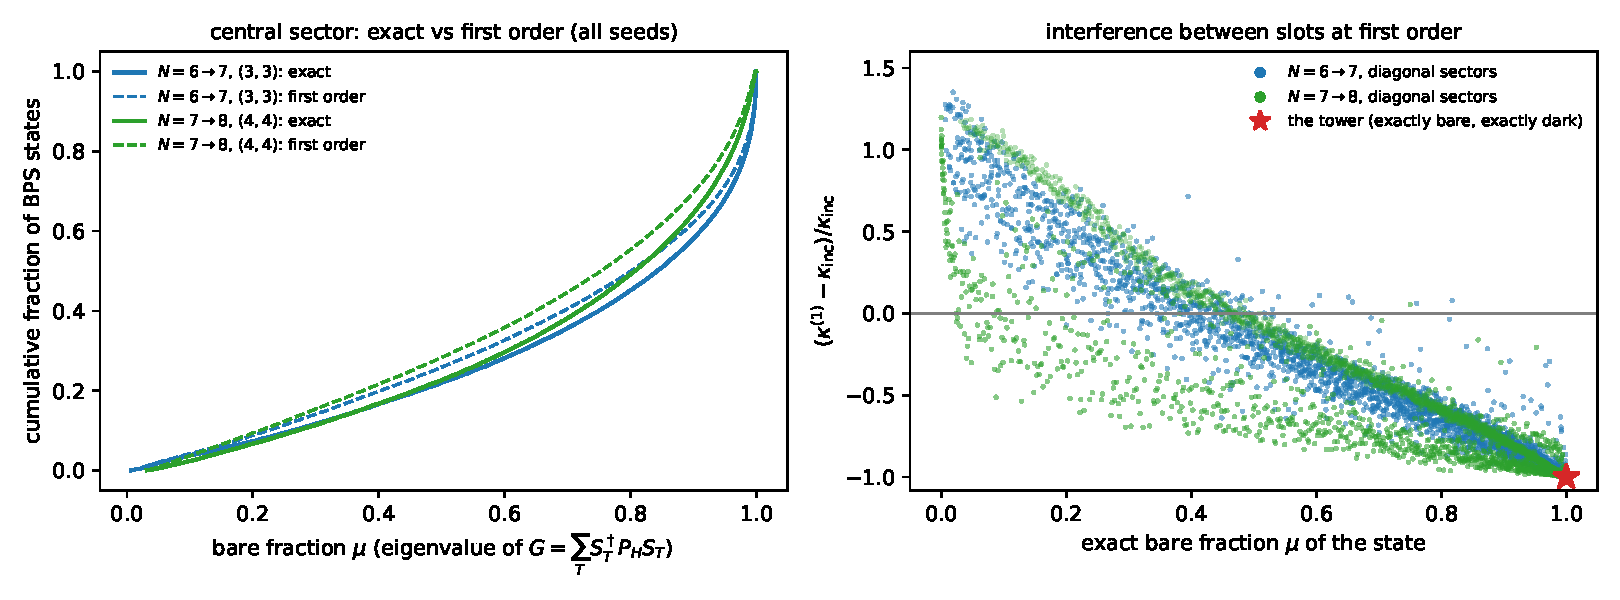
\includegraphics[width=\textwidth]{progress_2026-10-23_figs/fig_first_order.pdf}
\caption{(a) Cumulative distribution of the bare fraction $\mu$ in the central sector, exact (solid) vs.\ first order
(dashed). (b) Interference between slots at first order,
$(\kappa^{(1)}-\kappa_{\rm inc})/\kappa_{\rm inc}$, against the exact bare fraction for every dressed state of the
diagonal sectors. The tower (star) is exactly bare and exactly dark. \NUM}\label{fig:first}
\end{figure}

%=====================================================================
\section{The exact uplift in closed form}\label{sec:closed}
%=====================================================================

\emph{Added 25 October.} Sections~\ref{sec:onemode}--\ref{sec:pair} solved the pair uplift through an intermediate model
$M$, the old model plus $\psie$ alone, whose Hodge theory is not old-model data. This section removes $M$. Every object
below is built from the old model's BPS bases, its pseudo-inverses $Q_0^+$, $(Q_0^\dagger)^+$, its Green's operator
$G=H_0^+$, and the three couplings $E$, $K$, $Z$.

\paragraph{Notation.}
\begin{itemize}\itemsep2pt
\item Slot vectors are ordered by $w$: $\Psi=(\Psi_{01},\Psi_{00},\Psi_{11},\Psi_{10})$.
\item The new supercharge splits as $Q_{N+1}=Q_d+Q_c$. The slot-diagonal part is $Q_d=\mathrm{diag}(-Q_0,Q_0,Q_0,-Q_0)$.
  The cross-slot part $Q_c$ carries the arrows of Fig.~\ref{fig:slots}.
\item $\PH$ is the slotwise old harmonic projector, and $E_1=\bigoplus_T\B(\text{slot }T)$ is the old BPS data.
\end{itemize}

\subsection{Cohomology from old data: homological perturbation}

The triple (inclusion of $E_1$, projection $\PH$, homotopy $h=-Q_d^+$) is a strong deformation retract of the slotwise
complex. That is, $Q_dh+hQ_d=\iota\PH-1$ and $h^2=h\iota=\PH h=0$. The cross-slot part $Q_c$ raises $w$ while $h$
preserves it, so $(hQ_c)^3=0$. The homological perturbation lemma therefore applies with \emph{finite} series.

\begin{theorem}[Cohomology from old data]\label{thm:B}\VER\
$H(Q_{N+1})\cong H(E_1,D)$, with the transferred differential $D=\PH Q_c(1+Q_d^+Q_c)^{-1}\PH$:
\begin{equation}\label{eq:D}
D\eta=\big(0,\ \PH K\eta_{01},\ \PH E\eta_{01},\ \PH(E\eta_{00}-K\eta_{11}+\Zc\eta_{01})\big),\qquad
\Zc=Z-E\,Q_0^+K+K\,Q_0^+E .
\end{equation}
Hence $\dim\B_{N+1}(A,B)=\dim E_1(A,B)-\rk D_{(A,B)}-\rk D_{(A-2,B+1)}$.
\end{theorem}
\begin{proof}
The perturbation lemma gives $D=\PH Q_c(1-hQ_c)^{-1}\iota$, and the series stops at second order. The $w{+}1$ part of
$D$ is the slot complex $d_1$ of~\eqref{eq:slotcomplex}. The $w{+}2$ part is
$d_2=\PH(Z-EQ_0^+K+KQ_0^+E)\PH=\PH\Zc\PH$, and there are no higher terms. As a consistency check, the only
component of $D^2$ is $\PH(E\PH K-K\PH E)\PH=\PH[E,K]\PH=\PH\{Q_0,Z\}\PH=0$. The first equality uses the fact that
$(1-\PH)K$ maps harmonic forms to exact ones and $E$ keeps them exact.
\end{proof}

\VER\ There are no mismatches in any sector record: 950 symmetrized and 570 generic at $N\le6$, and 81 of each model at
$N=7$. The
$d_2$ of Table~\ref{tab:d2} is therefore no longer an obstacle: the old BPS data together with $\Zc$ determine the
enlarged BPS space exactly. $\Zc$ is a secondary, Massey-type operation. A bottom-slot class that $d_1$ annihilates
reaches the top slot either directly through the single-$\psi$ coupling $Z$, or by zig-zags through the dressed middle
slots, $EQ_0^+K$ and $KQ_0^+E$.

\subsection{BPS states in closed form}

\begin{theorem}[Closed-form BPS states]\label{thm:C}\VER\
Let $\Kc=Q_d^+Q_c+(Q_d^\dagger)^+Q_c^\dagger$. A slot vector $\Psi$ is BPS if and only if
\begin{equation}\label{eq:cf}
(1+\Kc)\Psi=\PH\Psi\qquad\text{and}\qquad \PH Q_c\Psi=0=\PH Q_c^\dagger\Psi .
\end{equation}
If $1+\Kc$ is invertible, then $\B_{N+1}=\{(1+\Kc)^{-1}h:\ h\in\mathcal A\}$ with
$\mathcal A=\ker\PH(Q_c\oplus Q_c^\dagger)(1+\Kc)^{-1}|_{E_1}$, and the four-slot harmonic map is injective.
\end{theorem}
\begin{proof}
($\Rightarrow$) Write $\Psi=h+r$ slotwise. $Q_{N+1}\Psi=0$ gives $Q_dr=-Q_c\Psi$. So $Q_c\Psi$ is exact, and the
coexact part of $r$ is $-Q_d^+Q_c\Psi$. Dually, the exact part of $r$ is $-(Q_d^\dagger)^+Q_c^\dagger\Psi$. Together
these say $r=-\Kc\Psi$.

($\Leftarrow$) From $(1+\Kc)\Psi=\PH\Psi$, $Q_{N+1}\Psi=(P_H+P_{\rm co})u$ with $u=Q_c\Psi$. Nilpotency gives
$Q_du=-Q_c(P_H+P_{\rm co})u$. Since $Q_c$ raises $w$, the lowest-$w$ component of $u$ is $Q_d$-closed. Its coexact part
therefore vanishes, and its harmonic part vanishes by assumption, so it is exact. Proceeding upward in $w$ shows
$Q_{N+1}\Psi=0$. The adjoint condition follows by downward induction.
\end{proof}

The ten blocks of $\Kc$ are explicit, e.g.\ $(00\leftarrow01)=Q_0^+K$, $(10\leftarrow00)=-Q_0^+E$,
$(01\leftarrow10)=-(Q_0^\dagger)^+Z^\dagger$. \VER\ At $N\le6$, in both models and all seeds:
\begin{itemize}\itemsep1pt
\item $(1+\Kc)^{-1}$ applied to the harmonic slot parts of each BPS state reconstructs it to $2\times10^{-13}$;
\item $\dim\mathcal A=\dim\B_{N+1}$ in every sector;
\item the closed-form states are BPS to $10^{-13}$.
\end{itemize}

\subsection{Integrating out the middle slots}

The dressing of the middle slots is explicit in the outer components:
$z_{00}=-Q_0^+K\Psi_{01}$, $x_{00}=-(Q_0^\dagger)^+E^\dagger\Psi_{10}$, $z_{11}=-Q_0^+E\Psi_{01}$ and
$x_{11}=(Q_0^\dagger)^+K^\dagger\Psi_{10}$. Substituting these leaves two equations of Dyson type for the outer slots.

\begin{proposition}[Reduced system]\label{prop:reduced}\VER\
The outer components of a BPS state satisfy
\begin{equation}\label{eq:dyson}
P_{\rm Co}(1+\SG)\Psi_{10}=Q_0^+\big(Eh_{00}-Kh_{11}+\Zc\Psi_{01}\big),\qquad
P_{\rm Ex}(1+\SGp)\Psi_{01}=(Q_0^\dagger)^+\big(K^\dagger h_{00}+E^\dagger h_{11}+\Zc'^\dagger\Psi_{10}\big),
\end{equation}
with the self-energies
\begin{equation}\label{eq:selfenergy}
\SG=E\,G\,E^\dagger+K\,G\,K^\dagger\ \ (\text{slot }10),\qquad \SGp=K^\dagger G\,K+E^\dagger G\,E\ \ (\text{slot }01).
\end{equation}
$\Zc'$ denotes $\Zc$ one charge level down. For the unknown dressing $u=(z_{10},x_{01})$ this is
$\Mb u=\sigma(h)$, with
\begin{equation}\label{eq:M}
\begin{gathered}
\Mb=\begin{pmatrix}1+\mathsf A&-L\\-L'&1+\mathsf A'\end{pmatrix},\\
\mathsf A=P_{\rm Co}\SG P_{\rm Co}\ge0,\quad \mathsf A'=P_{\rm Ex}\SGp P_{\rm Ex}\ge0,\quad L=Q_0^+\Zc,\quad
L'=(Q_0^\dagger)^+\Zc'^\dagger .
\end{gathered}
\end{equation}
The two off-diagonal blocks are related by $L'=-L^\dagger+C$, where the \emph{leak}
\begin{equation}\label{eq:leak}
\begin{gathered}
C=\alpha_{00}\gamma_{00}^\dagger-\alpha_{11}\gamma_{11}^\dagger,\\
\alpha_{00}=(Q_0^\dagger)^+K^\dagger\big|_{\B_{00}},\quad \gamma_{00}=Q_0^+E\big|_{\B_{00}},\quad
\alpha_{11}=(Q_0^\dagger)^+E^\dagger\big|_{\B_{11}},\quad \gamma_{11}=Q_0^+K\big|_{\B_{11}},
\end{gathered}
\end{equation}
factors through the BPS spaces $\B_{00}$, $\B_{11}$ of the middle slots.
\end{proposition}
\begin{proof}[Sketch]
The self-energy form of $\mathsf A$ follows from $\ip{z}{Q_0^+E(Q_0^\dagger)^+E^\dagger z}=\|P_{\rm ex}E^\dagger
v\|^2=\ip{z}{EGE^\dagger z}$ for $z=Q_0^\dagger v$, and the same with $E\to K$. Both forms are Hermitian, so they agree.
For the leak, $\{Q_0,Z\}=[E,K]$ together with $Q_0Q_0^+=P_{\rm ex}$ and $Q_0^+Q_0=P_{\rm co}$ gives
$\{Q_0,\Zc\}=E\PH K-K\PH E$. For $x=Q_0w$ and $z=Q_0^\dagger v$ this yields
$\ip{z}{Lx}+\ip{L'z}{x}=\ip{v}{(E\PH K-K\PH E)w}=\ip{z}{(\gamma_{00}\alpha_{00}^\dagger-\gamma_{11}\alpha_{11}^\dagger)x}$.
\end{proof}

\INTERP\ The middle slots act as virtual channels. Integrating them out leaves the outer slots with self-energies,
which are Euclidean-time-integrated two-point functions of $E$ and $K$ through the old continuum, and a transfer
amplitude $\Zc$. $\gamma_{00}h$ and $\alpha_{00}h$ are the first-order top- and bottom-slot dressings that a middle-slot
BPS state $h$ would create. The leak is the path ``top dressing $\to$ middle BPS state $\to$ bottom dressing''. It is
absent when the middle slots carry no BPS states. \VER\ $\mathsf A$, $\mathsf A'$ equal the projected self-energies,
and $L'+L^\dagger=C$ holds with the factorized $C$, both to $10^{-13}$.

\subsection{When is the uplift unique?}\label{sec:unique}

\begin{proposition}[Uniqueness criterion]\label{prop:unique}\DER\
$\mathrm{Herm}\,\Mb=1+\mathsf A\oplus\mathsf A'-\tfrac12\begin{pmatrix}0&C^\dagger\\C&0\end{pmatrix}$, so
$\mathrm{Herm}\,\Mb>0$ if and only if
$\rho:=\|(1+\mathsf A')^{-1/2}C(1+\mathsf A)^{-1/2}\|<2$. Then $\Mb$ is accretive and hence invertible. So are
$1+\Kc$ and the four-slot harmonic map, because the middle rows of $1+\Kc$ are explicit. Without middle cohomology,
$C=0$, $\mathrm{Herm}\,\Mb\ge1$ and $\|\Mb^{-1}\|\le1$, which is the contraction of the one-flavor uplift.
\end{proposition}

\NUM\ At unit coupling the criterion holds in $471$ of $499$ reduced systems (symmetrized) and $299$ of $319$ (generic)
at $N\le7$. $\Mb$ was invertible in all of them. At $N\le6$ the smallest $\sigma_{\min}(\Mb)$ is $0.31$ and $0.11$. At
$N=7$ (seed 1) it falls to $0.013$ in sectors $(3,3)$ and $(5,5)$ of the symmetrized model, and to $0.051$ in the generic
one. The old model there has a near-zero mode
(gap $0.0032$ in sector $(2,3)$), which inflates the dressing to $\|\Kc\|\approx150$. This is the origin of the bare
fraction $1.8\times10^{-6}$ noted in \S\ref{sec:pair}.

\paragraph{Injectivity is generic, not universal.} $\det\Mb$ is complex, so it can vanish on a set of codimension two in
coupling space. We scaled two independent families of the couplings that involve the new pair and minimized
$\sigma_{\min}(\Mb)$. This finds exact singular points in both models (Table~\ref{tab:pure}). At these points the BPS
dimension is unchanged, yet one BPS state has bare fraction zero: all four of its slot components are non-BPS states of
the old model. We call these \emph{pure-dressing} BPS states. In the symmetrized example the tower of the same sector
remains exactly bare. Four-slot injectivity, listed as an open problem in the first version of this report, is therefore
false in general. The correct statements are the criterion above and the two-step parametrization of
\S\ref{sec:pair}, which is a bijection everywhere.

\begin{table}[ht]
\centering\small
\caption{Exact pure-dressing BPS states at rescaled couplings, $N=4\to5$.
Generic: $g_1$ scales $C_{N i k}$, $C_{i N k}$ (the $E$ couplings) and $g_2$ scales $C_{ijN}$ (the $K$ couplings).
Symmetrized: $g_1$ scales $C_{N\cdot\cdot}$ and $g_2$ scales $C_{\cdot N\cdot}=C_{\cdot\cdot N}$.}\label{tab:pure}
\begin{tabular}{@{}lccccccc@{}}\toprule
model & seed & sector & $(g_1,g_2)$ & $\sigma_{\min}(\Mb)$ & $\dim\B_{N+1}$ & min.\ bare & deficit\\
 & & & & & & fraction & \\\midrule
generic & 2 & $(3,3)$ & $(0.4216,\,12.58)$ & $1.8\times10^{-16}$ & 65 & $\approx0$ & 1\\
symm. & 1 & $(2,2)$ & $(7.280,\,12.30)$ & $1.6\times10^{-16}$ & 65 & $\approx0$ & 1\\\bottomrule
\end{tabular}

\smallskip
{\small ``Deficit'' is the injectivity deficit of the four-slot harmonic map. In the symmetrized example the tower of
the same sector keeps bare fraction~1. Found and reproduced by \path{scripts/find_pure_dressing_states.py}.}
\end{table}

\subsection{Admissibility, slot weights and decoders}

\begin{proposition}[Admissibility and decoders]\label{prop:adm}\VER\
For $h\in E_1$, $\Psi=(1+\Kc)^{-1}h$ is BPS if and only if three conditions hold:
\begin{itemize}\itemsep2pt
\item[(a)] $\PH Kh_{01}=\PH Eh_{01}=0$ and $\PH E^\dagger h_{10}=\PH K^\dagger h_{10}=0$;
\item[(b)] $\PH(Eh_{00}^+-Kh_{11}^+ +\Zc h_{01})=0$, with $h_{00}^+=h_{00}+\alpha_{00}^\dagger x_{01}$ and
  $h_{11}^+=h_{11}+\alpha_{11}^\dagger x_{01}$;
\item[(c)] $\PH(K^\dagger h_{00}^-+E^\dagger h_{11}^-+\Zc'^\dagger h_{10})=0$, with
  $h_{00}^-=h_{00}+\gamma_{00}^\dagger z_{10}$ and $h_{11}^-=h_{11}-\gamma_{11}^\dagger z_{10}$.
\end{itemize}
Condition (b) says that the perturbation-lemma class representative $(h_{01},h_{00}^+,h_{11}^+,\cdot)$ of the state is a
$D$-cocycle; (c) is the dual statement. The slot weights of a BPS state are
\begin{gather}
\|\Psi_{01}\|^2=\|h_{01}\|^2+\|x_{01}\|^2,\qquad \|\Psi_{10}\|^2=\|h_{10}\|^2+\|z_{10}\|^2,\nonumber\\
\|\Psi_{00}\|^2=\|h_{00}\|^2+\ip{\Psi_{01}}{K^\dagger GK\Psi_{01}}+\ip{\Psi_{10}}{EGE^\dagger\Psi_{10}},\nonumber\\
\|\Psi_{11}\|^2=\|h_{11}\|^2+\ip{\Psi_{01}}{E^\dagger GE\Psi_{01}}+\ip{\Psi_{10}}{KGK^\dagger\Psi_{10}},
\label{eq:weights}
\end{gather}
and its dressing cost is $\kappa=\big[\|u\|^2+\ip{\Psi_{10}}{\SG\Psi_{10}}+\ip{\Psi_{01}}{\SGp\Psi_{01}}\big]/\|h\|^2$.
The bare-fraction decoder and CV's slot decoders are the generalized eigenvalue problems of
$(\|h\|^2,\|\Psi\|^2)$ and $(\|\Psi_T\|^2,\|\Psi\|^2)$ on $\mathcal A$.
\end{proposition}

The same four maps $\alpha$, $\gamma$ govern the leak~\eqref{eq:leak} and the corrections in (b), (c). The first-order
theory of \S\ref{sec:first} is the leading term: it drops the $\Mb$ corrections and replaces $\Psi_{10}$, $\Psi_{01}$
by $h_{10}$, $h_{01}$ inside $\kappa$. Two special cases are worth recording.
\begin{itemize}\itemsep2pt
\item One added mode: there are no middle slots, so $\mathsf A=\mathsf A'=0$ and $C=0$. $\Mb$ reduces to $1+$
  (anti-Hermitian), the one-flavor system.
\item The tower: $\Kc\eta=0$ and $\sigma(\eta)=0$ for $\eta=(0,V^n\Om,nV^{n-1}\Om,0)$, so $\Psi=\eta$ at every
  coupling.
\end{itemize}
\VER\ Conditions (a)--(c) give the same subspace as Theorem~\ref{thm:C} in every sector at $N\le6$. The pencils
reproduce the exact bare-fraction and slot-decoder spectra to $7\times10^{-13}$. At $N=7$ (one seed per model) all of
these checks hold to $2\times10^{-11}$; the larger residuals come from the nearly singular sectors of
\S\ref{sec:unique}.

\paragraph{Most of the exact correction is self-energy.} \NUM\ The closed form separates three levels of approximation.
\emph{First order} uses first-order sources and sets $\Mb\to1$ (\S\ref{sec:first}). \emph{Self-dressed} keeps the exact
sources and the self-energies, $\Mb\to1+\mathsf A\oplus\mathsf A'$, but drops the transfer and the leak. \emph{Exact}
solves the full system. On the exact admissible sources (sectors with at least 50 BPS states, $N=4$--$6$), self-dressing
moves the mean bare fraction from its first-order value $56$--$92\,\%$ of the way to the exact value. The median is
$0.67$ (symmetrized) and $0.79$ (generic). For example, in the central sector $(3,3)$ at $N=6\to7$ (five seeds) the
three levels are $0.7014$, $0.7220$ and $0.7322$. The direction is not always upward: in $(4,3)$ at $N=5\to6$ first order
is slightly high, and self-dressing corrects that too. The self-energies are pure time-integrated two-point functions
of $E$ and $K$, so a chord computation of those alone would capture most of the exact correction.
(\texttt{run\_two\_flavor\_uplift.py --tasks levels}.)

%=====================================================================
\section{Monotone versus fortuitous}\label{sec:summary}
%=====================================================================

Table~\ref{tab:mf} collects what the exact uplift says about the two kinds of states.

\begin{table}[ht]
\centering\small
\caption{What the uplift distinguishes.}\label{tab:mf}
\begin{tabular}{@{}>{\raggedright\arraybackslash}p{0.23\textwidth}>{\raggedright\arraybackslash}p{0.34\textwidth}>{\raggedright\arraybackslash}p{0.35\textwidth}@{}}\toprule
 & tower (monotone) & fortuitous\\\midrule
Hodge dressing & zero at every $N$ (bare), \VER & positive, except arithmetic walls in peripheral sectors, \NUM\\
mechanism & $J_{10}=J_{01}=0$ by $[E,V]=K$ & partial interference of $E$, $K$, $Z$ two-point functions\\
slot content & 00 and 11 only; weights $\frac{N+1-n}{N+1}$, $\frac{n}{N+1}$ & all admissible slots\\
bare-state count & the only excess over the generic count & equal to the generic count, same as generic couplings\\
CV channels 00, 11 & always exact (non-generic position) & exact iff $\dnew\ge R_T$ (generic position)\\
CV cost $\kappa_{00}$ & $=n/(N+1-n)$ iff $\dnew\le R_{00}$ & broad, growing (CV Fig.~8)\\
first-order dressing form & exactly dark & $O(1)$; interference from $+1$ to $\approx-1$\\
bare fraction over couplings & $=1$ for all couplings & in $[0,1)$; $=0$ (pure dressing) on a codimension-two set\\\bottomrule
\end{tabular}
\end{table}

\INTERP\ The two kinds of states differ in \emph{why} they survive the uplift. The tower survives by symmetry. Its uplift
is kinematical: old BPS states rearranged between slots, with all dressing currents cancelling by a Ward identity of the
$\mathfrak{su}(2)$ that generates it. CCSY call the $V$'s the analogue of gravitons, and the tower is the analogue of a
multi-graviton state built on the vacuum. Fortuitous states survive or fail by arithmetic, and when they survive they are
dressed. Their dressing is set by the old model's dynamics through Euclidean-time-integrated two-point functions. The
symmetrized and generic models are indistinguishable in all counting statistics, so the fortuitous sector does not ``know''
about the symmetry. Only the one state per diagonal sector that the symmetry singles out behaves differently.

%=====================================================================
\section{Discussion}\label{sec:discussion}
%=====================================================================

\subsection{What we have learned}

The one-flavor uplift at half filling was unobstructed: every old BPS state had an uplift, with a computable dressing
cloud. The two-flavor uplift is obstructed. Theorem~\ref{thm:A} shows that, once the obstruction is imposed on the
harmonic sources, the rest of the D6 structure survives intact: the anti-Hermitian system, the orthogonal splitting and
the minimum-norm uplift. The pair is two such steps. It also carries a genuinely new feature, the $d_2$ differential, so
the enlarged BPS space is not a function of old cohomology and first-order maps alone. The closed forms of
\S\ref{sec:closed} show what it \emph{is} a function of: the old BPS data; the self-energies $EGE^\dagger+KGK^\dagger$ and
$K^\dagger GK+E^\dagger GE$; the transfer $\Zc=Z-EQ_0^+K+KQ_0^+E$; and the four maps $\alpha$, $\gamma$ that connect the
middle-slot BPS states to the outer dressing.

Within this structure the monotone/fortuitous distinction is sharp and has a one-line origin, $[E,V]=K$. The tower is
the only state whose dressing currents vanish by an identity, at every $N$. The other bare states are arithmetic walls
that recede to peripheral sectors as $N$ grows. Everything else is arithmetic too:
\begin{itemize}\itemsep2pt
\item which fortuitous states lift exactly through which channel (Laws~\ref{law:L1}--\ref{law:L2});
\item which are bare (eq.~\eqref{eq:barelaw});
\item when the tower's channel cost reaches CV's bound (eq.~\eqref{eq:towercost}).
\end{itemize}
These laws are numerical, but they hold without exception outside $N=5$. Together they turn the structure of CV's
empirical Figs.~6, 7 and 9 into consequences of BPS dimensions and of the ranks of $Q_0$, $E$ and $K$.

\subsection{Towards Stage 2: what a chord computation must produce}

\INTERP\ Section~\ref{sec:first} identifies the objects. One flavor needed one two-point function, of the pair operator
$E=\eta\wedge$. Two flavors need three, of $\psi^\dagger\chi$, $\psi^\dagger\psi^\dagger$ and $\psi^\dagger$. They also
need their \emph{mixed} correlators, e.g.\ $\ip{Eh}{GKh'}$, which carry the interference. The monotone/fortuitous
distinction would then appear as follows:
\begin{itemize}\itemsep2pt
\item for the tower, a Ward identity making the mixed and diagonal terms cancel exactly;
\item for fortuitous states, the generic, partially cancelling spectrum of the same quadratic form.
\end{itemize}
D7 computed the one-flavor BPS$\to$continuum two-point function at fixed charge in closed form, an Al-Salam--Chihara
measure. A two-flavor version needs chord rules for two flavors with a charge lattice $(N_\psi,N_\chi)$. We have not
checked whether such rules exist in the literature; establishing that is the first task of Stage~2.

The closed forms of \S\ref{sec:closed} turn this into a definite list, valid exactly and not only at first order. The
exact uplift needs:
\begin{itemize}\itemsep2pt
\item the self-energies $\SG$, $\SGp$ (two-point functions of $E$ and $K$ through the old continuum);
\item the transfer $\Zc$ (the direct $Z$ coupling plus the zig-zags $EQ_0^+K$, $KQ_0^+E$);
\item the maps $\alpha$, $\gamma$ between middle-slot BPS states and the outer dressing.
\end{itemize}
A chord computation of these three ingredients would give the exact two-flavor uplift.

\subsection{Open problems}

\begin{enumerate}\itemsep2pt
\item The geometry of the singular set of $\Mb$ (pure-dressing states, \S\ref{sec:unique}). Does it approach unit
  coupling as $N$ grows?
\item Derivations of Laws~\ref{law:L1}--\ref{law:L2}, i.e.\ why the decoders are maximally generic inside their rooms.
  This is the analogue of CV's generic-position hypothesis, now with the refined rooms~\eqref{eq:rooms}.
\item The $N=5$ coincidences.
\item Simplifying the decoder pencils of Proposition~\ref{prop:adm} further, e.g.\ by push-through identities as in
  the one-flavor case.
\item Stage~2: the chord computation of $\SG$, $\SGp$, $\Zc$, $\alpha$ and $\gamma$.
\end{enumerate}

\appendix

%=====================================================================
\section{Verification summary}\label{app:verify}
%=====================================================================

\begin{table}[ht]
\centering\small
\caption{Checks of the exact statements (\texttt{tests/test\_two\_flavor.py}, 16 tests, and the production data). Residuals
are maxima.}\label{tab:verify}
\begin{tabular}{@{}>{\raggedright\arraybackslash}p{0.52\textwidth}>{\raggedright\arraybackslash}p{0.2\textwidth}l@{}}\toprule
Statement & Sizes & Residual\\\midrule
$Q^2=0$; $[Q,V]=0$ (symmetrized only); tower BPS, CV norms (86) & $N=4,5$ & $10^{-12}$\\
Block form~\eqref{eq:block} as an operator identity & $N=3$, both models & $10^{-12}$\\
$[Q_0,E]=[Q_0,K]=0$, $[E,K]=\{Q_0,Z\}$; $[E,V]=K$ (symmetrized) & $N=4$, both models & $10^{-12}$\\
Slot equations (Table~\ref{tab:slots}) on all BPS states & $N=4$, both models & $10^{-10}$\\
Theorem~\ref{thm:A} (step 1): admissible solve; obstructed residual; splitting & $N=4,5$, both models & $10^{-12}$; $\ge1$; $10^{-13}$\\
Two-step dimension formula~\eqref{eq:dimN} & $N=2$--$7$ & exact counts\\
Four-slot injectivity; reconstruction from harmonic parts & $N=2$--$7$ & deficit 0; $10^{-14}$\\
Tower bare, slot weights & $N=2$--$7$ & $4\times10^{-16}$\\
Single-slot first order $=$ two-point functions~\eqref{eq:sigmas} & $N=4$ & $10^{-8}$ (relative)\\
Tower dark at first order & $N=5$ & $10^{-10}$\\\midrule
\multicolumn{3}{@{}l}{\emph{Closed forms (added 25 October)}}\\
$\dim\B_{N+1}=\dim H(E_1,D)$ (Theorem~\ref{thm:B}) & $N=2$--$7$, both models & exact counts\\
$(1+\Kc)^{-1}$ reconstructs BPS states; $\dim\mathcal A=\dim\B_{N+1}$; BPS residual & $N=2$--$7$, both models & $2\times10^{-12}$; exact; $10^{-12}$\\
Self-energy form of $\mathsf A$, $\mathsf A'$; $L'+L^\dagger=C$, factorized leak & $N=3$--$6$, both models & $10^{-13}$\\
Admissibility (a)--(c) $=$ Theorem~\ref{thm:C}; decoder pencils & $N=3$--$6$ (pencils $N\le7$) & exact; $2\times10^{-11}$\\
Herm$\,\Mb\ge1-\|C\|/2$ & $N=2$--$7$, both models & no violation\\\bottomrule
\end{tabular}
\end{table}

%=====================================================================
\section{Numerical methods and reproducibility}\label{app:repro}
%=====================================================================

\begin{itemize}\itemsep1pt
\item Couplings: \texttt{rng = default\_rng(seed)}, with $G$ i.i.d.\ complex Gaussian, $\mathbb E|G|^2=2$.
\item Symmetrized couplings $C=(G+G^{T_{jk}})/2$: function \texttt{random\_symmetric\_couplings}.
\item Generic couplings $C=G$: function \texttt{random\_generic\_couplings}.
\item The old model is the restriction of the $(N+1)$-pair couplings to the first $N$ pairs; the new pair sits at the
  top two bits of the Fock basis.
\item All linear algebra is dense. BPS spaces are kernels of the Laplacian with relative tolerance $10^{-9}$.
\item Seeds: symmetrized $1$--$5$ ($N=2$--$6$) and $1$--$2$ ($N=7$); generic $1$--$3$ ($N=2$--$6$) and $1$ ($N=7$).
\item All runs used \path{scripts/memwatch.py}; the largest peak among completed runs was $3.65$\,GB, at $N=7$. A first seed-1 job at $N=7$ cached all first-order
pseudo-inverses; it was stopped at $4.6$\,GB, before writing any first-order records, and the first-order and tower
tasks were rerun with per-sector cache release (\path{research/notes/two_flavor_uplift_2026-10-23.md}).
\end{itemize}

\begin{center}\small
\begin{tabular}{@{}>{\raggedright\arraybackslash}p{0.3\textwidth}>{\raggedright\arraybackslash}p{0.65\textwidth}@{}}\toprule
Item & Code and data\\\midrule
Model; uplift machinery & \path{src/two_flavor.py}, \path{src/two_flavor_uplift.py}; tests \path{tests/test_two_flavor.py}\\
Production runs & \path{scripts/run_two_flavor_uplift.py} (tasks \texttt{dims cv bare first tower e2 closed}) $\to$ \path{results/data/two_flavor_2026-10-23/*.jsonl}, logs, metadata\\
Pure-dressing states & \path{scripts/find_pure_dressing_states.py} $\to$ \path{pure_dressing_*.json}\\
Analysis, tables, figures & \path{scripts/analyze_two_flavor_uplift.py} $\to$ \path{summary.json}, \path{results/figures/two_flavor_2026-10-23/}\\
Derivations; research note & \path{docs/derivations.md} D8; \path{research/notes/two_flavor_uplift_2026-10-23.md}\\\bottomrule
\end{tabular}
\end{center}

\begin{thebibliography}{99}\small
\bibitem{CV} J.~Chryssanthacopoulos and D.~Vegh, \emph{Fortuity and fragility in supersymmetric SYK}, arXiv:2608.12160 (2026).
\bibitem{CCSY} C.-M.~Chang, Y.~Chen, B.~S.~Sia and Z.~Yang, \emph{Fortuity in SYK models}, arXiv:2412.06902.
\bibitem{HTZ} M.~Heydeman, G.~J.~Turiaci and W.~Zhao, \emph{Phases of $\mathcal N=2$ Sachdev-Ye-Kitaev models}, arXiv:2206.14900.
\bibitem{prog1013} \texttt{syk\_gravity} project, \emph{Progress report, 13 October 2026: the uplift map and the origin of localization}, \path{research/pdfs/progress_2026-10-13.pdf}.
\bibitem{prog1014} \texttt{syk\_gravity} project, \emph{Progress report, 14 October 2026: the dressing spectrum from chords}, \path{research/pdfs/progress_2026-10-14.pdf}.
\end{thebibliography}

\end{document}
